\documentclass[aspectratio=169]{beamer}\usepackage[]{graphicx}\usepackage[]{xcolor}
% maxwidth is the original width if it is less than linewidth
% otherwise use linewidth (to make sure the graphics do not exceed the margin)
\makeatletter
\def\maxwidth{ %
  \ifdim\Gin@nat@width>\linewidth
    \linewidth
  \else
    \Gin@nat@width
  \fi
}
\makeatother

\definecolor{fgcolor}{rgb}{0.345, 0.345, 0.345}
\newcommand{\hlnum}[1]{\textcolor[rgb]{0.686,0.059,0.569}{#1}}%
\newcommand{\hlsng}[1]{\textcolor[rgb]{0.192,0.494,0.8}{#1}}%
\newcommand{\hlcom}[1]{\textcolor[rgb]{0.678,0.584,0.686}{\textit{#1}}}%
\newcommand{\hlopt}[1]{\textcolor[rgb]{0,0,0}{#1}}%
\newcommand{\hldef}[1]{\textcolor[rgb]{0.345,0.345,0.345}{#1}}%
\newcommand{\hlkwa}[1]{\textcolor[rgb]{0.161,0.373,0.58}{\textbf{#1}}}%
\newcommand{\hlkwb}[1]{\textcolor[rgb]{0.69,0.353,0.396}{#1}}%
\newcommand{\hlkwc}[1]{\textcolor[rgb]{0.333,0.667,0.333}{#1}}%
\newcommand{\hlkwd}[1]{\textcolor[rgb]{0.737,0.353,0.396}{\textbf{#1}}}%
\let\hlipl\hlkwb

\usepackage{framed}
\makeatletter
\newenvironment{kframe}{%
 \def\at@end@of@kframe{}%
 \ifinner\ifhmode%
  \def\at@end@of@kframe{\end{minipage}}%
  \begin{minipage}{\columnwidth}%
 \fi\fi%
 \def\FrameCommand##1{\hskip\@totalleftmargin \hskip-\fboxsep
 \colorbox{shadecolor}{##1}\hskip-\fboxsep
     % There is no \\@totalrightmargin, so:
     \hskip-\linewidth \hskip-\@totalleftmargin \hskip\columnwidth}%
 \MakeFramed {\advance\hsize-\width
   \@totalleftmargin\z@ \linewidth\hsize
   \@setminipage}}%
 {\par\unskip\endMakeFramed%
 \at@end@of@kframe}
\makeatother

\definecolor{shadecolor}{rgb}{.97, .97, .97}
\definecolor{messagecolor}{rgb}{0, 0, 0}
\definecolor{warningcolor}{rgb}{1, 0, 1}
\definecolor{errorcolor}{rgb}{1, 0, 0}
\newenvironment{knitrout}{}{} % an empty environment to be redefined in TeX

\usepackage{alltt}

% Set lecture number for later use


% Part common to all the lectures
\subtitle{MATH 8xyz -- Lecture 23}
\author{\texorpdfstring{Julien Arino\newline Department of Mathematics @ University of Manitoba \newline Maud Menten Institute @ PIMS\newline\url{julien.arino@umanitoba.ca}}{Julien Arino}}
\date{Winter 20XX}

% Title of the lecture
\title{Models using continuous-time Markov chains}



\usetheme{default}
% Slide setup, colour independent

\usepackage{amsmath,amssymb,amsthm}
\usepackage[utf8]{inputenc}
\usepackage{colortbl}
\usepackage{bm}
\usepackage{xcolor}
\usepackage{dsfont}
\usepackage{setspace}
% To use \ding{234} and the like
\usepackage{pifont}
% To cross reference between slide files
\usepackage{zref-xr,zref-user}
% Use something like
% \zexternaldocument{fileI}
% in the tex files. And cite using \zref instead of \ref
\usepackage{booktabs}
\usepackage{marvosym}
\usepackage{cancel}
%\usepackage{transparent}
% Make doi clickable in the bibliography?
\usepackage{doi}

\usepackage[T1]{fontenc}

\usepackage{longtable}

% For heavier titles
\usepackage{helvet} % Enables Helvetica font family


% Fields and the like
\def\IC{\mathbb{C}}
\def\IE{\mathbb{E}}
\def\IF{\mathbb{F}}
\def\II{\mathbb{I}}
\def\IJ{\mathbb{J}}
\def\IK{\mathbb{K}}
\def\IM{\mathbb{M}}
\def\IN{\mathbb{N}}
\def\IP{\mathbb{P}}
\def\IR{\mathbb{R}}
\newcommand{\IRplus}{\mathbb{R}_{\ge 0}}
\def\IZ{\mathbb{Z}}
\def\11{\mathds{1}}


% Bold lowercase
\def\ba{\bm{a}}
\def\bb{\bm{b}}
\def\bc{\bm{c}}
\def\bd{\bm{d}}
\def\be{\bm{e}}
\def\bf{\bm{f}}
\def\bg{\bm{g}}
\def\bh{\bm{h}}
\def\bi{\bm{i}}
\def\bj{\bm{j}}
\def\bk{\bm{k}}
\def\bn{\bm{n}}
\def\bp{\bm{p}}
\def\br{\bm{r}}
\def\bs{\bm{s}}
\def\bu{\bm{u}}
\def\bv{\bm{v}}
\def\bw{\bm{w}}
\def\bx{\bm{x}}
\def\by{\bm{y}}
\def\bz{\bm{z}}
\newcommand{\vect}[1]{\bm{#1}}

% Bold capitals
\def\bB{\bm{B}}
\def\bD{\bm{D}}
\def\bE{\bm{E}}
\def\bF{\bm{F}}
\def\bG{\bm{G}}
\def\bI{\bm{I}}
\def\bL{\bm{L}}
\def\bN{\bm{N}}
\def\bP{\bm{P}}
\def\bR{\bm{R}}
\def\bS{\bm{S}}
\def\bT{\bm{T}}
\def\bX{\bm{X}}

% Bold numbers
\def\b0{\bm{0}}

% Bold greek
\bmdefine{\bmu}{\bm{\mu}}
\def\bphi{\bm{\phi}}
\def\bvarphi{\bm{\varphi}}
\def\bPi{\bm{\Pi}}
\def\bGamma{\bm{\Gamma}}

% Bold red sentence
\def\boldred#1{{\color{red}\textbf{#1}}}
\def\defword#1{{\color{orange}\textbf{#1}}}

% Caligraphic letters
\def\A{\mathcal{A}}
\def\B{\mathcal{B}}
\def\C{\mathcal{C}}
\def\D{\mathcal{D}}
\def\E{\mathcal{E}}
\def\F{\mathcal{F}}
\def\G{\mathcal{G}}
\def\H{\mathcal{H}}
\def\I{\mathcal{I}}
\def\L{\mathcal{L}}
\def\M{\mathcal{M}}
\def\N{\mathcal{N}}
\def\P{\mathcal{P}}
\def\R{\mathcal{R}}
\def\S{\mathcal{S}}
\def\T{\mathcal{T}}
\def\U{\mathcal{U}}
\def\V{\mathcal{V}}

% Adding space for prime (') where needed
\def\pprime{\,'}
% Adding space for star (\star) where needed
\def\pstar{{\,\star}}

% tt font for code
\def\code#1{{\tt #1}}

% i.e., e.g.
\def\eg{\emph{e.g.}}
\def\ie{\emph{i.e.}}


% Operators and special symbols
\def\nbOne{{\mathchoice {\rm 1\mskip-4mu l} {\rm 1\mskip-4mu l}
{\rm 1\mskip-4.5mu l} {\rm 1\mskip-5mu l}}}
\def\cov{\ensuremath{\mathsf{cov}}}
\def\Var{\ensuremath{\mathsf{Var}\ }}
\def\Im{\textrm{Im}\;}
\def\Re{\textrm{Re}\;}
\def\det{\ensuremath{\mathsf{det}}}
\def\diag{\ensuremath{\mathsf{diag}}}
\def\nullspace{\ensuremath{\mathsf{null}}}
\def\nullity{\ensuremath{\mathsf{nullity}}}
\def\rank{\ensuremath{\mathsf{rank}}}
\def\range{\ensuremath{\mathsf{range}}}
\def\sgn{\ensuremath{\mathsf{sgn}}}
\def\Span{\ensuremath{\mathsf{span}}}
\def\tr{\ensuremath{\mathsf{tr}}}
\def\imply{$\Rightarrow$}
\def\restrictTo#1#2{\left.#1\right|_{#2}}
\newcommand{\parallelsum}{\mathbin{\!/\mkern-5mu/\!}}
\def\dsum{\mathop{\displaystyle \sum }}%
\def\dind#1#2{_{\substack{#1\\ #2}}}

\newcommand{\Qmatrix}[1]{%
  \begin{pmatrix}#1\end{pmatrix}%
}

\DeclareMathOperator{\GL}{GL}
\DeclareMathOperator{\Rel}{Re}
\def\Nt#1{\left|\!\left|\!\left|#1\right|\!\right|\!\right|}
\newcommand{\tripbar}{|\! |\! |}



% The beamer bullet (in base colour)
\def\bbullet{\leavevmode\usebeamertemplate{itemize item}\ }

% Theorems and the like
\newtheorem{proposition}[theorem]{Proposition}
\newtheorem{property}[theorem]{Property}
\newtheorem{importantproperty}[theorem]{Property}
\newtheorem{importanttheorem}[theorem]{Theorem}
%\newtheorem{lemma}[theorem]{Lemma}
%\newtheorem{corollary}[theorem]{Corollary}
\newtheorem{remark}[theorem]{Remark}
\setbeamertemplate{theorems}[numbered]
%\setbeamertemplate{theorems}[ams style]

%
%\usecolortheme{orchid}
%\usecolortheme{orchid}

\def\red{\color[rgb]{1,0,0}}
\def\blue{\color[rgb]{0,0,1}}
\def\green{\color[rgb]{0,1,0}}

% Fix skipping lines after items in the bibliography
\setbeamertemplate{bibliography entry title}{}
\setbeamertemplate{bibliography entry location}{}
\setbeamertemplate{bibliography entry note}{}

% Get rid of navigation stuff
\setbeamertemplate{navigation symbols}{}

% Set footline/header line
\setbeamertemplate{footline}
{%
\quad p. \insertpagenumber \quad--\quad \insertsection\vskip2pt
}
% \setbeamertemplate{headline}
% {%
% \quad\insertsection\hfill p. \insertpagenumber\quad\mbox{}\vskip2pt
% }


\makeatletter
\newlength\beamerleftmargin
\setlength\beamerleftmargin{\Gm@lmargin}
\makeatother

% Colours for special pages
\def\extraContent{yellow!20}


%%%%%%%%%%%%%%%%%
\usepackage{tikz}
\usetikzlibrary{shapes,arrows}
\usetikzlibrary{positioning}
\usetikzlibrary{shapes.symbols,shapes.callouts,patterns}
\usetikzlibrary{calc,fit}
\usetikzlibrary{backgrounds}
\usetikzlibrary{decorations.pathmorphing,fit,petri}
\usetikzlibrary{automata}
\usetikzlibrary{fadings}
\usetikzlibrary{patterns,hobby}
\usetikzlibrary{backgrounds,fit,petri}
\usetikzlibrary{tikzmark}

\usepackage{pgfplots}
\pgfplotsset{compat=1.6}
\pgfplotsset{ticks=none}

\usetikzlibrary{decorations.markings}
\usetikzlibrary{arrows.meta}
\tikzset{>=stealth}

% For tikz
\tikzstyle{cloud} = [draw, ellipse,fill=red!20, node distance=0.87cm,
minimum height=2em]
\tikzstyle{line} = [draw, -latex']


%%% For max frame images
\newenvironment{changemargin}[2]{%
\begin{list}{}{%
\setlength{\topsep}{0pt}%
\setlength{\leftmargin}{#1}%
\setlength{\rightmargin}{#2}%
\setlength{\listparindent}{\parindent}%
\setlength{\itemindent}{\parindent}%
\setlength{\parsep}{\parskip}%
}%
\item[]}{\end{list}}


% Make one image take up the entire slide content area in beamer,.:
% centered/centred full-screen image, with title:
% This uses the whole screen except for the 1cm border around it
% all. 128x96mm
\newcommand{\titledFrameImage}[2]{
\begin{frame}{#1}
%\begin{changemargin}{-1cm}{-1cm}
\begin{center}
\includegraphics[width=108mm,height=\textheight,keepaspectratio]{#2}
\end{center}
%\end{changemargin}
\end{frame}
}

% Make one image take up the entire slide content area in beamer.:
% centered/centred full-screen image, no title:
% This uses the whole screen except for the 1cm border around it
% all. 128x96mm
\newcommand{\plainFrameImage}[1]{
\begin{frame}[plain]
%\begin{changemargin}{-1cm}{-1cm}
\begin{center}
\includegraphics[width=108mm,height=76mm,keepaspectratio]{#1}
\end{center}
%\end{changemargin}
\end{frame}
}

% Make one image take up the entire slide area, including borders, in beamer.:
% centered/centred full-screen image, no title:
% This uses the entire whole screen
\newcommand{\maxFrameImage}[1]{
\begin{frame}[plain]
\begin{changemargin}{-1cm}{-1cm}
\begin{center}
\includegraphics[width=\paperwidth,height=\paperheight,keepaspectratio]
{#1}
\end{center}
\end{changemargin}
\end{frame}
}

% This uses the entire whole screen (to include in frame)
\newcommand{\maxFrameImageNoFrame}[1]{
\begin{changemargin}{-1cm}{-1cm}
\begin{center}
\includegraphics[width=\paperwidth,height=0.99\paperheight,keepaspectratio]
{#1}
\end{center}
\end{changemargin}
}

% Make one image take up the entire slide area, including borders, in beamer.:
% centered/centred full-screen image, no title:
% This uses the entire whole screen
\newcommand{\maxFrameImageColor}[2]{
\begin{frame}[plain]
\setbeamercolor{normal text}{bg=#2!20}
\begin{changemargin}{-1cm}{-1cm}
\begin{center}
\includegraphics[width=\paperwidth,height=\paperheight,keepaspectratio]
{#1}
\end{center}
\end{changemargin}
\end{frame}
}


\usepackage{tikz}
\usetikzlibrary{patterns,hobby}
\usepackage{pgfplots}
\pgfplotsset{compat=1.6}
\pgfplotsset{ticks=none}

\usetikzlibrary{backgrounds}
\usetikzlibrary{decorations.markings}
\usetikzlibrary{arrows.meta}
\tikzset{>=stealth}

\tikzset{
  clockwise arrows/.style={
    postaction={
      decorate,
      decoration={
        markings,
        mark=between positions 0.1 and 0.9 step 40pt with {\arrow{>}},
   }}}}


% Beginning of a section
\newcommand{\newSectionSlide}[1]{
\begin{frame}[noframenumbering,plain]
  \begin{tikzpicture}[remember picture,overlay]
    \node[above right,inner sep=0pt,opacity=0.2] at (current page.south west)
    {
        \includegraphics[height=\paperheight,width=\paperwidth]{#1}
    };
  \end{tikzpicture}
  \setbeamercolor{section in toc}{fg=section_page_list_colour}
  \setbeamerfont{section in toc}{size=\Large,series=\bfseries}
  \setbeamertemplate{section in toc shaded}[default][60]
  \tableofcontents[
    currentsection,
    sectionstyle=show/shaded,
    subsectionstyle=show/hide/hide,
    subsubsectionstyle=hide/hide/hide]
\end{frame}
\addtocounter{page}{-1}
}

% Beginning of a section in which we also show subsections
\newcommand{\newSectionWithSubsSlide}[1]{
	\begin{frame}[noframenumbering,plain]
		\begin{tikzpicture}[remember picture,overlay]
			\node[above right,inner sep=0pt,opacity=0.2] at (current page.south west)
			{
				\includegraphics[height=\paperheight,width=\paperwidth]{#1}
			};
		\end{tikzpicture}
		\setbeamercolor{section in toc}{fg=section_page_list_colour}
		\setbeamerfont{section in toc}{size=\Large,series=\bfseries}
		\setbeamertemplate{section in toc shaded}[default][60]
		\tableofcontents[
		currentsection,
		sectionstyle=show/hide,
		subsectionstyle=show/show/hide,
		subsubsectionstyle=hide/hide/hide]
	\end{frame}
	\addtocounter{page}{-1}
}

% Beginning of a subsection
\newcommand{\newSubSectionSlide}[1]{
\begin{frame}[noframenumbering,plain]
  \begin{tikzpicture}[remember picture,overlay]
    \node[above right,inner sep=0pt,opacity=0.2] at (current page.south west)
    {
        \includegraphics[height=\paperheight,width=\paperwidth]{#1}
    };
  \end{tikzpicture}
  \setbeamercolor{section in toc}{fg=subsection_page_list_colour}
  \setbeamerfont{section in toc}{size=\Large,series=\bfseries}
  \setbeamertemplate{section in toc shaded}[default][60]
  \setbeamerfont{subsection in toc}{series=\bfseries}
  \setbeamertemplate{subsection in toc shaded}[default][50]
  \tableofcontents[
    currentsection,
    sectionstyle=show/hide,
    subsectionstyle=show/shaded/hide,
    subsubsectionstyle=hide/hide/hide]
\end{frame}
\addtocounter{page}{-1}
}


% Beginning of a subsubsection
\newcommand{\newSubSubSectionSlide}[1]{
\begin{frame}[noframenumbering,plain]
  \begin{tikzpicture}[remember picture,overlay]
    \node[above right,inner sep=0pt,opacity=0.2] at (current page.south west)
    {
        \includegraphics[height=\paperheight,width=\paperwidth]{#1}
    };
  \end{tikzpicture}
  \setbeamercolor{section in toc}{fg=subsub_header_section}
  \setbeamerfont{section in toc}{size=\Large,series=\bfseries}
  \setbeamertemplate{section in toc shaded}[default][60]
  \setbeamerfont{subsection in toc}{series=\bfseries}
  \setbeamertemplate{subsection in toc shaded}[default][50]
  \setbeamertemplate{subsubsection in toc shaded}[default][50]
  \tableofcontents[
    currentsection,
    sectionstyle=show/hide,
    subsectionstyle=show/hide/hide,
    subsubsectionstyle=show/shaded/hide]
\end{frame}
\addtocounter{page}{-1}
}


   %%%%%%%%%%%
% To have links to parts in the outline
\makeatletter
\AtBeginPart{%
  \addtocontents{toc}{\protect\beamer@partintoc{\the\c@part}{\beamer@partnameshort}{\the\c@page}}%
}
%% number, shortname, page.
\providecommand\beamer@partintoc[3]{%
  \ifnum\c@tocdepth=-1\relax
    % requesting onlyparts.
    \makebox[6em]{Part #1:} \textcolor{green!30!blue}{\hyperlink{#2}{#2}}
    \par
  \fi
}
\define@key{beamertoc}{onlyparts}[]{%
  \c@tocdepth=-1\relax
}
\makeatother%

\newcommand{\nameofthepart}{}
\newcommand{\nupart}[1]%
    {   \part{#1}%
        \renewcommand{\nameofthepart}{#1}%
        {
          \setbeamercolor{background canvas}{bg=orange!50}
          \begin{frame}{#1}%\partpage 
          \hypertarget{\nameofthepart}{}\tableofcontents%
          \end{frame}
        }
    }

% This command creates a title page using TikZ only
\newcommand{\tikztitlepage}[1]{%
\begin{frame}[plain,noframenumbering]
  \begin{tikzpicture}[remember picture,overlay]
    % Background image
    \node[above right,inner sep=0pt,opacity=0.1] 
      at (current page.south west) 
      {\includegraphics[width=\paperwidth,height=\paperheight]{#1}};

    % University logo
    \node[anchor=north east, inner sep=5pt, opacity=0.9] 
      at (current page.north east)
      {
\includegraphics[width=0.2\textwidth]{FIGS-slides-admin/UM-logo-horizontal-CMYK.png}};
    
    % Title
    \node[anchor=center, align=center, 
          font=\fontsize{13}{15}\bfseries\color{UMbrown}, 
          text width=0.9\textwidth] 
          at ([yshift=2cm]current page.center)
          {\inserttitle};

      % Authors
      \node[anchor=center, align=center,
        font=\fontsize{10}{12}\bfseries\color{UMbrown},
        text width=0.7\textwidth]
        at ([yshift=0.8cm]current page.center)
        {\insertauthor};

      % Affiliation
      \node[anchor=north, align=center,
        font=\fontsize{9}{11}\color{UMbrown},
        text width=0.7\textwidth]
        at ([yshift=-0.2cm]current page.center)
        {\insertaffiliation};      
    % Date
    \node[anchor=north, align=center, 
          font=\fontsize{12}{16}\bfseries\color{UMbrown},
          text width=0.7\textwidth] 
          at ([yshift=0.2cm]current page.center)
          {\insertdate};

    % Land acknowledgement
    \node[anchor=south, align=justify, 
          font=\footnotesize, text=black, 
          text width=1.1\textwidth] 
          at ([yshift=0.5cm]current page.south)
          {The University of Manitoba campuses are located on original lands of Anishinaabeg, Ininew, Anisininew, Dakota and Dene peoples, and on the National Homeland of the Red River Métis.\\
          We respect the Treaties that were made on these territories, we acknowledge the harms and mistakes of the past, and we dedicate ourselves to move forward in partnership with Indigenous communities in a spirit of Reconciliation and collaboration.};
  \end{tikzpicture}
  \addtocounter{page}{-1}
\end{frame}
}
% The title page with figure
% \newcommand{\titlepagewithfigure}[1]{%
%   \begin{frame}[noframenumbering,plain]
%     \begin{tikzpicture}[remember picture,overlay]
%       \node[above right,inner sep=0pt,opacity=0.1] at (current page.south west)
%       {
%           \includegraphics[height=\paperheight,width=\paperwidth]{#1}
%       };
%       \node[anchor=north east,
%       inner sep=5pt,
%       opacity=0.9] at (current page.north east)
%       {
%           
\includegraphics[width=0.2\textwidth]{FIGS-slides-admin/UM-logo-horizontal-CMYK.png}
%       };
%       \node[anchor=south, 
%       align=justify, 
%       text=black, 
%       text width=1.1\textwidth,
%       font=\footnotesize]  (land_acknowledgement)
%       at (current page.south) 
%       {The University of Manitoba campuses are located on original lands of Anishinaabeg, Ininew, Anisininew, Dakota and Dene peoples, and on the National Homeland of the Red River Métis.
%       We respect the Treaties that were made on these territories, we acknowledge the harms and mistakes of the past, and we dedicate ourselves to move forward in partnership with Indigenous communities in a spirit of Reconciliation and collaboration.};  
%       % \node[align=center, anchor=south,
%       % above=0.5cm of land_acknowledgement,
%       % text=black,
%       % font=\bfseries] {\insertdate};
%   \end{tikzpicture}
%   \setbeamercolor{title}{fg=title_page_title_colour}
%   \setbeamerfont{title}{size=\Large,series=\bfseries}
%   \setbeamercolor{author}{fg=title_page_author_colour}
%   \setbeamerfont{author}{size=\large,series=\bfseries}
%   \setbeamercolor{institute}{fg=title_page_institute_colour}
%   \setbeamerfont{institute}{size=\large,series=\bfseries}
%   \setbeamercolor{date}{fg=title_page_date_colour}
%   \setbeamerfont{date}{series=\bfseries}
% 	\titlepage
% \end{frame}
% \addtocounter{page}{-1}
% }

\newcommand{\titlepagewithfigure}[1]{%
  \begin{frame}[noframenumbering,plain]
    \begin{tikzpicture}[remember picture,overlay]
      \node[above right,inner sep=0pt,opacity=0.1] at (current page.south west)
      {
          \includegraphics[height=\paperheight,width=\paperwidth]{#1}
      };
      \node[anchor=north east,
      inner sep=5pt,
      opacity=0.9] at (current page.north east)
      {
          
\includegraphics[width=0.2\textwidth]{FIGS-slides-admin/UM-logo-horizontal-CMYK.png}
      };
      \node[anchor=south, 
      align=justify, 
      text=black, 
      text width=1.1\textwidth,
      font=\footnotesize]  (land_acknowledgement)
      at (current page.south) 
      {The University of Manitoba campuses are located on original lands of Anishinaabeg, Ininew, Anisininew, Dakota and Dene peoples, and on the National Homeland of the Red River Métis.
      We respect the Treaties that were made on these territories, we acknowledge the harms and mistakes of the past, and we dedicate ourselves to move forward in partnership with Indigenous communities in a spirit of Reconciliation and collaboration.};  
      % \node[align=center, anchor=south,
      % above=0.5cm of land_acknowledgement,
      % text=black,
      % font=\bfseries] {\insertdate};
  \end{tikzpicture}
  \setbeamercolor{title}{fg=title_page_title_colour}
  \setbeamerfont{title}{size=\Large,series=\bfseries,family=\usefont{T1}{phv}{b}{n}}
  \setbeamercolor{author}{fg=title_page_author_colour}
  \setbeamerfont{author}{size=\large,series=\bfseries,family=\usefont{T1}{phv}{b}{n}}
  \setbeamercolor{institute}{fg=title_page_institute_colour}
  \setbeamerfont{institute}{size=\large,series=\bfseries,family=\usefont{T1}{phv}{b}{n}}
  \setbeamercolor{date}{fg=title_page_date_colour}
  \setbeamerfont{date}{series=\bfseries,family=\usefont{T1}{phv}{b}{n}}
	\titlepage
\end{frame}
\addtocounter{page}{-1}
}
% The outline page, with figure
% \newcommand{\outlinepage}[1]{%
% \begin{frame}[noframenumbering,plain]
%   \begin{tikzpicture}[remember picture,overlay]
%     \node[above right,inner sep=0pt,opacity=0.2] at (current page.south west)
%     {
%         \includegraphics[height=\paperheight,width=\paperwidth]{#1}
%     };
%   \end{tikzpicture}
%   \setbeamercolor{section in toc}{fg=outline_page_list_colour}
%   \setbeamerfont{section in toc}{size=\Large,series=\bfseries,family=\sffamily}
%   \frametitle{\textcolor{outline_page_title_colour}{\LARGE\bfseries Outline}}
%   \tableofcontents[hideallsubsections]
% \end{frame}
% \addtocounter{page}{-1}
% }
% The outline page, with figure
\newcommand{\outlinepage}[1]{%
\begin{frame}[noframenumbering,plain]
  \begin{tikzpicture}[remember picture,overlay]
    \node[above right,inner sep=0pt,opacity=0.2] at (current page.south west)
    {
        \includegraphics[height=\paperheight,width=\paperwidth]{#1}
    };
  \end{tikzpicture}
  \setbeamercolor{section in toc}{fg=outline_page_list_colour}
  % Use Helvetica Bold only for the outline slide TOC
  \setbeamerfont{section in toc}{size=\Large,family=\usefont{T1}{phv}{b}{n}}
  % Use Helvetica Bold for the outline title
  \frametitle{\textcolor{outline_page_title_colour}{\usefont{T1}{phv}{b}{n}\LARGE Outline}}
  \tableofcontents[hideallsubsections]
\end{frame}
\addtocounter{page}{-1}
}


%\let\oldsection\section
%\renewcommand{\section}[2]{\oldsection[#1]\newSectionSlide[#2]}





\usecolortheme{orchid}
%% Listings
\usepackage{listings}
\definecolor{mygreen}{rgb}{0,0.6,0}
\definecolor{mygray}{rgb}{0.5,0.5,0.5}
\definecolor{mymauve}{rgb}{0.58,0,0.82}
\definecolor{mygold}{rgb}{1,0.843,0}
\definecolor{myblue}{rgb}{0.537,0.812,0.941}

\definecolor{mygold2}{RGB}{120,105,22}
\definecolor{mygrey2}{RGB}{50,50,50}

\definecolor{lgreen}{rgb}{0.6,0.9,.6}
\definecolor{lred}{rgb}{1,0.5,.5}

\lstloadlanguages{R}
\lstset{ %
  language=R,
  backgroundcolor=\color{black!05},   % choose the background color
  basicstyle=\footnotesize\ttfamily,        % size of fonts used for the code
  breaklines=true,                 % automatic line breaking only at whitespace
  captionpos=b,                    % sets the caption-position to bottom
  commentstyle=\color{mygreen},    % comment style
  escapeinside={\%*}{*)},          % if you want to add LaTeX within your code
  keywordstyle=\color{red},       % keyword style
  stringstyle=\color{mygold},     % string literal style
  keepspaces=true,
  columns=fullflexible,
  tabsize=4,
}
% Could also do (in lstset)
% basicstyle==\fontfamily{pcr}\footnotesize
\lstdefinelanguage{Renhanced}%
  {keywords={abbreviate,abline,abs,acos,acosh,action,add1,add,%
      aggregate,alias,Alias,alist,all,anova,any,aov,aperm,append,apply,%
      approx,approxfun,apropos,Arg,args,array,arrows,as,asin,asinh,%
      atan,atan2,atanh,attach,attr,attributes,autoload,autoloader,ave,%
      axis,backsolve,barplot,basename,besselI,besselJ,besselK,besselY,%
      beta,binomial,body,box,boxplot,break,browser,bug,builtins,bxp,by,%
      c,C,call,Call,case,cat,category,cbind,ceiling,character,char,%
      charmatch,check,chol,chol2inv,choose,chull,class,close,cm,codes,%
      coef,coefficients,co,col,colnames,colors,colours,commandArgs,%
      comment,complete,complex,conflicts,Conj,contents,contour,%
      contrasts,contr,control,helmert,contrib,convolve,cooks,coords,%
      distance,coplot,cor,cos,cosh,count,fields,cov,covratio,wt,CRAN,%
      create,crossprod,cummax,cummin,cumprod,cumsum,curve,cut,cycle,D,%
      data,dataentry,date,dbeta,dbinom,dcauchy,dchisq,de,debug,%
      debugger,Defunct,default,delay,delete,deltat,demo,de,density,%
      deparse,dependencies,Deprecated,deriv,description,detach,%
      dev2bitmap,dev,cur,deviance,off,prev,,dexp,df,dfbetas,dffits,%
      dgamma,dgeom,dget,dhyper,diag,diff,digamma,dim,dimnames,dir,%
      dirname,dlnorm,dlogis,dnbinom,dnchisq,dnorm,do,dotplot,double,%
      download,dpois,dput,drop,drop1,dsignrank,dt,dummy,dump,dunif,%
      duplicated,dweibull,dwilcox,dyn,edit,eff,effects,eigen,else,%
      emacs,end,environment,env,erase,eval,equal,evalq,example,exists,%
      exit,exp,expand,expression,External,extract,extractAIC,factor,%
      fail,family,fft,file,filled,find,fitted,fivenum,fix,floor,for,%
      For,formals,format,formatC,formula,Fortran,forwardsolve,frame,%
      frequency,ftable,ftable2table,function,gamma,Gamma,gammaCody,%
      gaussian,gc,gcinfo,gctorture,get,getenv,geterrmessage,getOption,%
      getwd,gl,glm,globalenv,gnome,GNOME,graphics,gray,grep,grey,grid,%
      gsub,hasTsp,hat,heat,help,hist,home,hsv,httpclient,I,identify,if,%
      ifelse,Im,image,\%in\%,index,influence,measures,inherits,install,%
      installed,integer,interaction,interactive,Internal,intersect,%
      inverse,invisible,IQR,is,jitter,kappa,kronecker,labels,lapply,%
      layout,lbeta,lchoose,lcm,legend,length,levels,lgamma,library,%
      licence,license,lines,list,lm,load,local,locator,log,log10,log1p,%
      log2,logical,loglin,lower,lowess,ls,lsfit,lsf,ls,machine,Machine,%
      mad,mahalanobis,make,link,margin,match,Math,matlines,mat,matplot,%
      matpoints,matrix,max,mean,median,memory,menu,merge,methods,min,%
      missing,Mod,mode,model,response,mosaicplot,mtext,mvfft,na,nan,%
      names,omit,nargs,nchar,ncol,NCOL,new,next,NextMethod,nextn,%
      nlevels,nlm,noquote,NotYetImplemented,NotYetUsed,nrow,NROW,null,%
      numeric,\%o\%,objects,offset,old,on,Ops,optim,optimise,optimize,%
      options,or,order,ordered,outer,package,packages,page,pairlist,%
      pairs,palette,panel,par,parent,parse,paste,path,pbeta,pbinom,%
      pcauchy,pchisq,pentagamma,persp,pexp,pf,pgamma,pgeom,phyper,pico,%
      pictex,piechart,Platform,plnorm,plogis,plot,pmatch,pmax,pmin,%
      pnbinom,pnchisq,pnorm,points,poisson,poly,polygon,polyroot,pos,%
      postscript,power,ppoints,ppois,predict,preplot,pretty,Primitive,%
      print,prmatrix,proc,prod,profile,proj,prompt,prop,provide,%
      psignrank,ps,pt,ptukey,punif,pweibull,pwilcox,q,qbeta,qbinom,%
      qcauchy,qchisq,qexp,qf,qgamma,qgeom,qhyper,qlnorm,qlogis,qnbinom,%
      qnchisq,qnorm,qpois,qqline,qqnorm,qqplot,qr,Q,qty,qy,qsignrank,%
      qt,qtukey,quantile,quasi,quit,qunif,quote,qweibull,qwilcox,%
      rainbow,range,rank,rbeta,rbind,rbinom,rcauchy,rchisq,Re,read,csv,%
      csv2,fwf,readline,socket,real,Recall,rect,reformulate,regexpr,%
      relevel,remove,rep,repeat,replace,replications,report,require,%
      resid,residuals,restart,return,rev,rexp,rf,rgamma,rgb,rgeom,R,%
      rhyper,rle,rlnorm,rlogis,rm,rnbinom,RNGkind,rnorm,round,row,%
      rownames,rowsum,rpois,rsignrank,rstandard,rstudent,rt,rug,runif,%
      rweibull,rwilcox,sample,sapply,save,scale,scan,scan,screen,sd,se,%
      search,searchpaths,segments,seq,sequence,setdiff,setequal,set,%
      setwd,show,sign,signif,sin,single,sinh,sink,solve,sort,source,%
      spline,splinefun,split,sqrt,stars,start,stat,stem,step,stop,%
      storage,strstrheight,stripplot,strsplit,structure,strwidth,sub,%
      subset,substitute,substr,substring,sum,summary,sunflowerplot,svd,%
      sweep,switch,symbol,symbols,symnum,sys,status,system,t,table,%
      tabulate,tan,tanh,tapply,tempfile,terms,terrain,tetragamma,text,%
      time,title,topo,trace,traceback,transform,tri,trigamma,trunc,try,%
      ts,tsp,typeof,unclass,undebug,undoc,union,unique,uniroot,unix,%
      unlink,unlist,unname,untrace,update,upper,url,UseMethod,var,%
      variable,vector,Version,vi,warning,warnings,weighted,weights,%
      which,while,window,write,\%x\%,x11,X11,xedit,xemacs,xinch,xor,%
      xpdrows,xy,xyinch,yinch,zapsmall,zip},%
   otherkeywords={!,!=,~,$,*,\%,\&,\%/\%,\%*\%,\%\%,<-,<<-,_,/},%
   alsoother={._$},%
   sensitive,%
   morecomment=[l]\#,%
   morestring=[d]",%
   morestring=[d]'% 2001 Robert Denham
  }%

%%%%%%% 
%% Definitions in yellow boxes
\usepackage{etoolbox}
\setbeamercolor{block title}{use=structure,fg=structure.fg,bg=structure.fg!40!bg}
\setbeamercolor{block body}{parent=normal text,use=block title,bg=block title.bg!20!bg}

\BeforeBeginEnvironment{definition}{%
	\setbeamercolor{block title}{fg=black,bg=yellow!20!white}
	\setbeamercolor{block body}{fg=black, bg=yellow!05!white}
}
\AfterEndEnvironment{definition}{
	\setbeamercolor{block title}{use=structure,fg=structure.fg,bg=structure.fg!20!bg}
	\setbeamercolor{block body}{parent=normal text,use=block title,bg=block title.bg!50!bg, fg=black}
}
\BeforeBeginEnvironment{importanttheorem}{%
	\setbeamercolor{block title}{fg=black,bg=red!20!white}
	\setbeamercolor{block body}{fg=black, bg=red!05!white}
}
\AfterEndEnvironment{importanttheorem}{
	\setbeamercolor{block title}{use=structure,fg=structure.fg,bg=structure.fg!20!bg}
	\setbeamercolor{block body}{parent=normal text,use=block title,bg=block title.bg!50!bg, fg=black}
}
\BeforeBeginEnvironment{importantproperty}{%
	\setbeamercolor{block title}{fg=black,bg=red!50!white}
	\setbeamercolor{block body}{fg=black, bg=red!30!white}
}
\AfterEndEnvironment{importantproperty}{
	\setbeamercolor{block title}{use=structure,fg=structure.fg,bg=structure.fg!20!bg}
	\setbeamercolor{block body}{parent=normal text,use=block title,bg=block title.bg!50!bg, fg=black}
}

% Colour for the outline page
\definecolor{outline_colour}{RGB}{230,165,83}
%% Colours for sections, subsections aand subsubsections
\definecolor{section_colour}{RGB}{27,46,28}
\definecolor{subsection_colour}{RGB}{52,128,56}
\definecolor{subsubsection_colour}{RGB}{150,224,154}
\definecolor{subsub_header_section}{RGB}{196,44,27}
%\definecolor{mygold}{rgb}{1,0.843,0}
% Beginning of a section
% \AtBeginSection[]{
% 	{
% 	  \setbeamercolor{section in toc}{fg=mygold}
% 		\setbeamercolor{background canvas}{bg=section_colour}
% 		\begin{frame}[noframenumbering,plain]
% 			\framesubtitle{\nameofthepart Chapter \insertromanpartnumber \ -- \iteminsert{\insertpart}}
% 			\tableofcontents[
% 				currentsection,
% 				sectionstyle=show/shaded,
% 				subsectionstyle=show/hide/hide,
% 				subsubsectionstyle=hide/hide/hide]
% 		\end{frame}
% 	\addtocounter{page}{-1}
% 	%\addtocounter{framenumber}{-1} 
% 	}
% }


% % Beginning of a section
% \AtBeginSubsection[]{
% 	{
% 	  \setbeamercolor{section in toc}{fg=mygold}
% 		\setbeamercolor{background canvas}{bg=subsection_colour}
% 		\begin{frame}[noframenumbering,plain]
% 				\framesubtitle{\nameofthepart Chapter \insertromanpartnumber \ -- \iteminsert{\insertpart}}
% 				\tableofcontents[
% 					currentsection,
% 					sectionstyle=show/hide,
% 					currentsubsection,
% 					subsectionstyle=show/shaded/hide,
% 					subsubsectionstyle=show/hide/hide]
% 			\end{frame}
% 		\addtocounter{page}{-1}
% 	}
% }

% \newcommand{\newSubSectionSlide}[1]{
% \begin{frame}[noframenumbering,plain]
%   \begin{tikzpicture}[remember picture,overlay]
%     \node[above right,inner sep=0pt,opacity=0.2] at (current page.south west)
%     {
%         \includegraphics[height=\paperheight,width=\paperwidth]{#1}
%     };
%   \end{tikzpicture}
%   \setbeamercolor{section in toc}{fg=subsub_header_section}
%   \setbeamerfont{section in toc}{size=\Large,series=\bfseries}
%   \setbeamertemplate{section in toc shaded}[default][60]
%   \setbeamertemplate{subsection in toc shaded}[default][60]
%   %\setbeamercolor{background canvas}{bg=section_colour}
%   \tableofcontents[
%     currentsection,
%     sectionstyle=show/hide,
%     currentsubsection,
%     subsectionstyle=show/shaded/hide,
%     subsubsectionstyle=show/hide/hide]
% \end{frame}
% \addtocounter{page}{-1}
% }


% % Beginning of a section
% \AtBeginSubsubsection[]{
% 	{
% 	  \setbeamercolor{section in toc}{fg=subsub_header_section}
% 	  \setbeamercolor{subsubsection in toc}{fg=mygold2}
% 	  \setbeamercolor{subsubsection in toc shaded}{fg=mygrey2}
% 		\setbeamercolor{background canvas}{bg=subsubsection_colour}
% 		\begin{frame}[noframenumbering,plain]
% 				\framesubtitle{\nameofthepart Chapter \insertromanpartnumber \ -- \iteminsert{\insertpart}}
% 				\tableofcontents[
% 					currentsection,
% 					sectionstyle=show/hide,
% 					currentsubsection,
% 					subsectionstyle=show/hide/shaded
% 					currentsubsubsection]%,
% 					%subsubsectionstyle=hide/hide/shaded]
% 					%currentsubsubsection]
% 			\end{frame}
% 		\addtocounter{page}{-1}
% 	}
% }


\IfFileExists{upquote.sty}{\usepackage{upquote}}{}
\begin{document}

%%%%%%%%%%%%%%%%%%%%%%%%%%%%%%%%%
%%%%%%%%%%%%%%%%%%%%%%%%%%%%%%%%%
%% TITLE AND OUTLINE
%%%%%%%%%%%%%%%%%%%%%%%%%%%%%%%%%
%%%%%%%%%%%%%%%%%%%%%%%%%%%%%%%%%
\titlepagewithfigure{FIGS-slides-admin/Gemini_Generated_Image_uckjmbuckjmbuckj.jpeg}
\outlinepage{FIGS-slides-admin/Gemini_Generated_Image_sq8p8jsq8p8jsq8p.jpeg}


%%%%%%%%%%%%%%%%%%%
%%%%%%%%%%%%%%%%%%%
%%%%%%%%%%%%%%%%%%%
%%%%%%%%%%%%%%%%%%%
\section{Why incorporate stochasticity?}
% The section page
\newSectionSlide{FIGS-slides-admin/Gemini_Generated_Image_tve93ftve93ftve9.jpeg}

\begin{frame}{At the beginning of the COVID-19 crisis}
\bbullet 
I was working under contract with the Public Health Agency of Canada on \emph{COVID-19 importation risk assessment}
\vfill
\bbullet 
Produced daily report with list of countries most likely to next report cases of COVID-19
\vfill
\bbullet
Used ensemble runs of a fitted global deterministic metapopulation model
\end{frame}

\maxFrameImage{FIGS/covid-cluster}

\begin{frame}
\bbullet Very very long days (18-20 hours, 7 days a week)
\vfill
\bbullet including a lot of time waiting for the ``cluster'' to finish
\vfill
$\implies$ PHAC gave me money for a cluster (yay Threadrippers!!!)
\vfill
$\implies$ Also thought about whether my model was really adequate as our focus switched from thinking about movement on a planetary scale to movement within Canadian provinces
\end{frame}

\begin{frame}{What is wrong with deterministic models?}
\bbullet I pointed out yesterday that SARS-CoV-2 is one \emph{single} realisation of a stochastic process
\vfill
\bbullet Deterministic models ``operate on averages'' over a large ($\to\infty$) number of realisations
\vfill
\bbullet If we want to get a better sense of what could happen, not only on average, then we need to see what can indeed happen
\end{frame}

\begin{frame}{My new focus -- Introductions}
\bbullet I started thinking in particular about \defword{introductions} (or importations) of pathogens into new populations
\vfill
\bbullet Indeed, introductions are an obligatory step in spatial spread
\end{frame}

\begin{frame}{First piece of evidence}
In real life, introductions of pathogens does not always follow the patter
\begin{center}
\{$\R_0<1 \implies \to$ DFE | $\R_0>1 \implies $ epidemic or $\to$ EEP\} 
\end{center}
\end{frame}

\maxFrameImage{FIGS/Delory_etal-cover}
\maxFrameImage{FIGS/Delory_etal-table}

\begin{frame}{Second piece of evidence}
The start of an outbreak can be extremely slow, with very few cases for quite a while
\end{frame}

\maxFrameImage{FIGS/select_Wyoming-Campbell_bars_zoom}

\begin{frame}{Why this is relevant}
Far from the only reason, but as an example: Canada has remote/isolated communities that are vulnerable to introductions of pathogens
\end{frame}

\maxFrameImage{FIGS/cities_roads_CAN-MB_detail.png}
\maxFrameImage{FIGS/nutrition-north-canada-eligibility.png}
\maxFrameImage{FIGS/Screenshot from 2024-06-25 14-42-25.png}
\maxFrameImage{FIGS/Screenshot from 2024-06-25 16-56-16.png}

\begin{frame}{For First Nation and Métis Communities}
  \defword{Remote} describes a \textbf{geographical area} where a community is \textbf{located over 350 km} from the \textbf{nearest service centre} \textbf{having year-round access} by land and/or water routes normally used in all weather conditions
  \vfill	
  \defword{Isolated} means a \textbf{geographical area} that has \textbf{scheduled flights} and good telephone service, but is \textbf{without year-round access} by land and/or water normally used in all weather conditions
  \vfill
  \defword{Remote-Isolated} means a \textbf{geographic area} that has \textbf{neither scheduled flights nor year-round access} by land and/or water routes normally that can be used in all weather conditions, irrespective of the level of telephone and radio service available
\end{frame}

\begin{frame}{For Inuit communities}
  Inuit Communities to be referred to as \defword{Inuit Nunangat}, not remote and isolated communities to respect the unique language and culture of Inuit regions, as well as the common challenges in social determinants of health, access to care, and infrastructure found across all Inuit communities
\end{frame}

\begin{frame}\frametitle{MB remote communities}
  \begin{quote}
  \defword{Remote communities} are communities in Manitoba that \textbf{do not have permanent road access} (i.e., no all-weather road), are \textbf{more than a four-hour drive} from a major rural hospital (and a dialysis unit), \textbf{or have rail or fly-in access only}. This includes Norway House, Lynn Lake, Leaf Rapids, Gillam, and Cross Lake. If most communities in a health district are designated as "remote", the entire district is designated as "remote". In Manitoba, remote districts include:
  \begin{itemize}
  \item Northern Health Region: NO23, NO13, NO25, NO16, NO22, NO26, NO28, NO31, and
  \item Interlake-Eastern Health Region: IE61.
  \end{itemize}
  \end{quote}
  \vfill
  \small
  Chartier M, Dart A, Tangri N, Komenda P, Walld R, Bogdanovic B, Burchill C, Koseva I, McGowan K, Rajotte L. Care of Manitobans Living with Chronic Kidney Disease. Winnipeg, MB.
  Manitoba Centre for Health Policy, December 2015
\end{frame}

\maxFrameImage{FIGS/remote-health-regions.png}

\begin{frame}{Travel to/from remote or isolated communities}
  How do you think this compares to travel in non-remote/isolated communities ?
  \vfill
  Residence time (the lake ecology version): theoretic time an average water or comparable molecule spends in a lake, considering inflow into and outflow from the lake
  \vfill
  Think of residence times in these communities: what is the average time a person spends in a remote or isolated community before leaving it?
  \vfill
  The \defword{residence time in a location} is the total number of trips inbound into and outbound from location over a duration of time (1 month here) divided by the normal population in the location 
\end{frame}

\maxFrameImage{FIGS/residence-time-in-airports.png}

\begin{frame}{The paradox of travel to/from remote/isolated communities}
Travel volumes small but movement rates high
\vfill
ICs are highly connected to the urban centre(s) they are subordinated to
\vfill
Further reinforced in Winnipeg by urban indigenous population (102,075 or 12.45\% of metro population), meaning many family connections exist
\end{frame}

% \begin{frame}{Travel restrictions/interruptions}
% During COVID, travelling above 53 north in MB was forbidden for anyone not resident above 53 north	
% \vfill
% If you wanted to fly to Nunavut, you needed to spend two weeks in quarantine in a hotel in Edmonton, Ottawa or Winnipeg
% \vfill
% Canada implemented two weeks quarantine when IB from abroad (with exceptions)
% \vfill
% Canada interrupted travel from a variety of places
% \end{frame}
% 
% 
% \begin{frame}\frametitle{Questions}
% 	\begin{itemize}
% 		\item What is the probability that an introduction is successful? \newline (note: I am judging things from the perspective of the pathogen)
% 		\vfill
% 		\item How long is the stochastic phase following an introduction?
% 		\newline (what Amy called the ``stuttering period'')
% 		\vfill
% 		\item What do the different control measures do, how good are they?
% 	\end{itemize}
% \end{frame}



%%%%%%%%%%%%%%%%%%%
%%%%%%%%%%%%%%%%%%%
%%%%%%%%%%%%%%%%%%%
%%%%%%%%%%%%%%%%%%%
\section{Stochasticity in deterministic models}
% The section page
\newSectionSlide{FIGS-slides-admin/Gemini_Generated_Image_5yvymh5yvymh5yvy.jpeg}


\subsection{Distributions of times to events}
% The section page
\newSubSectionSlide{FIGS-slides-admin/Gemini_Generated_Image_fu32wbfu32wbfu32.jpeg}

\begin{frame}
See in particular the work of \href{https://scholar.google.ca/citations?user=o7R6ZHMAAAAJ}{Horst Thieme}
\vfill
If one considers time of sojourn in compartments from a more detailed perspective, one obtains integro-differential models
\vfill
We use here continuous random variables. See chapters 12 and 13 in \href{https://press.princeton.edu/books/paperback/9780691092911/mathematics-in-population-biology}{Thieme's book} for arbitrary distributions
\end{frame}


\begin{frame}\frametitle{Time to events}
We suppose that a system can be in two states, $A$ and $B$
\begin{itemize}
\item At time $t=0$, the system is in state $A$
\item An event happens at some time $t=\tau$, which triggers the switch from
state $A$ to state $B$
\end{itemize}
\vfill
Let us call $T$ the random variable 
\begin{quote}
``time spent in state $A$ before switching into state $B$''
\end{quote}
\end{frame}

\begin{frame}
The states can be anything:
\begin{itemize}
\item $A$: working, $B$: broken
\item $A$: infected, $B$: recovered
\item $A$: alive, $B$: dead
\item $\ldots$
\end{itemize}
\vfill
We take a collection of objects or individuals that are in state $A$ and want
some law for the \defword{distribution} of the times spent in $A$, i.e., a law for $T$
\vfill
For example, we make light bulbs and would like to tell our customers that on average, our light bulbs last 200 years...
\vfill
We conduct an \defword{infinite} number of experiments, and observe the time that it takes, in every experiment, to switch from $A$ to $B$
\end{frame}

\begin{frame}
\begin{center}
  \begin{tikzpicture}[auto, %node distance = 2cm, auto,
  scale=0.8, every node/.style={transform shape},
  cloud/.style={minimum width={width("XN-1")+2pt},
  draw, ellipse,fill=blue!20}]
  \node [cloud] (S0_1) at (0,0) {$A$};
  \node [cloud] (S1_1) at (2,0) {$B$};
  \node [cloud] (S0_2) at (0,-1) {$A$};
  \node [cloud] (S1_2) at (2.5,-1) {$B$};
  \node [cloud] (S0_3) at (0,-2) {$A$};
  \node [cloud] (S1_3) at (3.5,-2) {$B$};
  \node [cloud] (S0_4) at (0,-3) {$A$};
  \node [cloud] (S1_4) at (1.5,-3) {$B$};
  %%
  \node [cloud] (S0_10) at (0,-5) {$A$};
  \node [cloud] (S1_10) at (5.5,-5) {$B$};
  %%
  \node [cloud] (S0_15) at (0,-7) {$A$};
  \node [cloud] (S1_15) at (5,-7) {$B$};
  %% Arrows
  \path [line, very thick] (S0_1) to (S1_1);
  \path [line, very thick] (S0_2) to (S1_2);
  \path [line, very thick] (S0_3) to (S1_3);
  \path [line, very thick] (S0_4) to (S1_4);
  \path [line, very thick] (S0_10) to (S1_10);
  \path [line, very thick] (S0_15) to (S1_15);
  %%
  \draw [-,-, dashed, thick] (S0_4) -- (S0_10);
  \draw [-,-, dashed, thick] (S0_10) to (S0_15);
  \draw [-,-, dashed, thick] (S0_15) to (0,-8);
  %% The time arrow
  \path [line, very thick] (0,-8.35) to (7,-8.35);
  \node[anchor=north, align=center,text=black] at (6,-8.5)
  {time}; 
  \node[anchor=north, align=center,text=black] at (0,-8.5)
  {$0$}; 
  \end{tikzpicture}
\end{center}
\end{frame}


\begin{frame}\frametitle{A distribution of probability is a model}
From the sequence of experiments, we deduce a model, which in this context is called a \defword{probability distribution}
\vfill
We assume that $T$ is a \defword{continuous} random variable
\end{frame}



\begin{frame}\frametitle{Probability density function}
Since $T$ is continuous, it has a continuous \defword{probability density function} $f$
\begin{minipage}{0.4\textwidth}
\begin{itemize}
\item $f\geq 0$
\item $\int_{-\infty}^{+\infty}f(s)ds=1$
\item $\IP(a\leq T\leq b)=\int_a^bf(t)dt$
\end{itemize}
\end{minipage}
\begin{minipage}{0.59\textwidth}
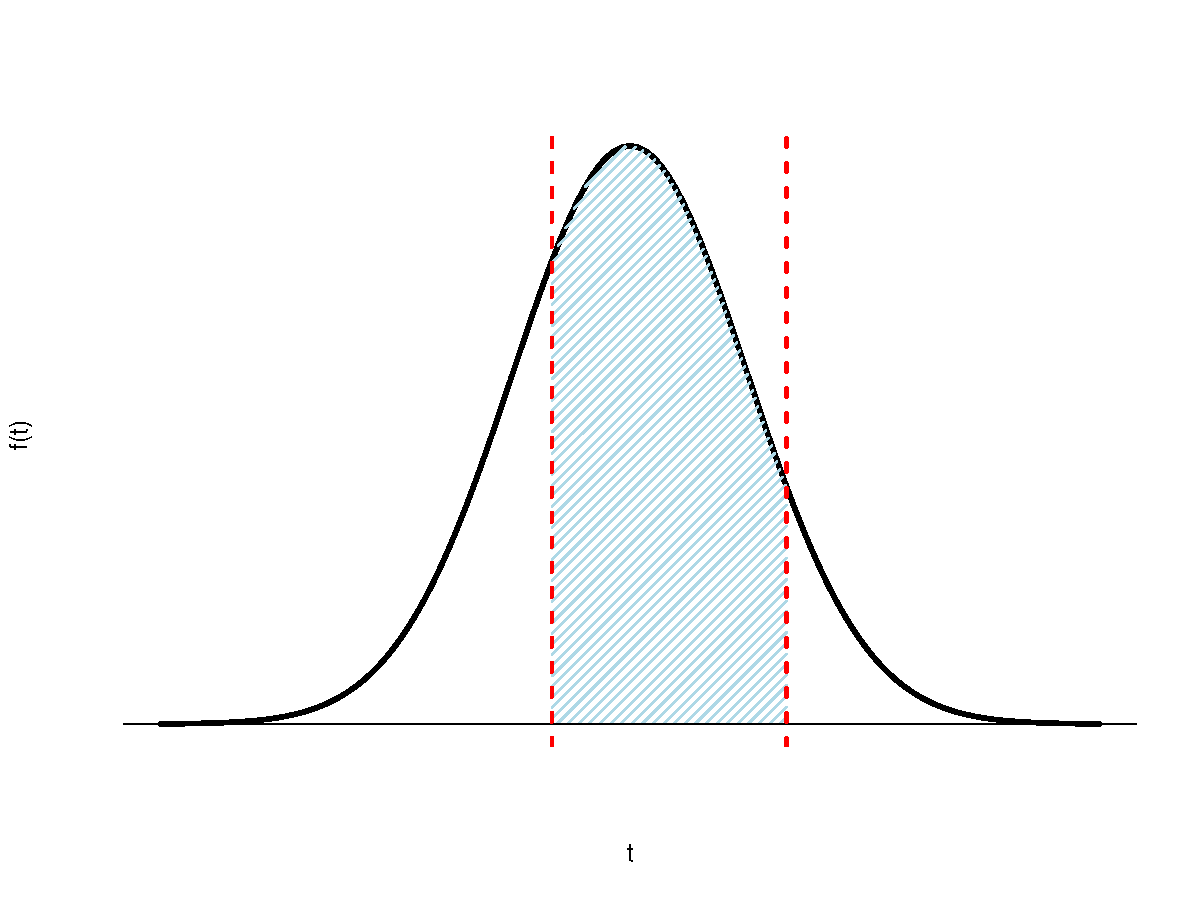
\includegraphics[width=\textwidth]{FIGS/L23-distrib_a_b-1.pdf}
\end{minipage}
\end{frame}



\begin{frame}\frametitle{Cumulative distribution function (c.d.f.)}
\begin{minipage}{0.4\textwidth}
The \defword{cumulative distribution function} is a function $F(t)$ that characterizes the distribution of $T$, and defined by
\[
F(s)=\IP(T\leq s)=\int_{-\infty}^sf(x)dx
\]
\end{minipage}
\begin{minipage}{0.59\textwidth}
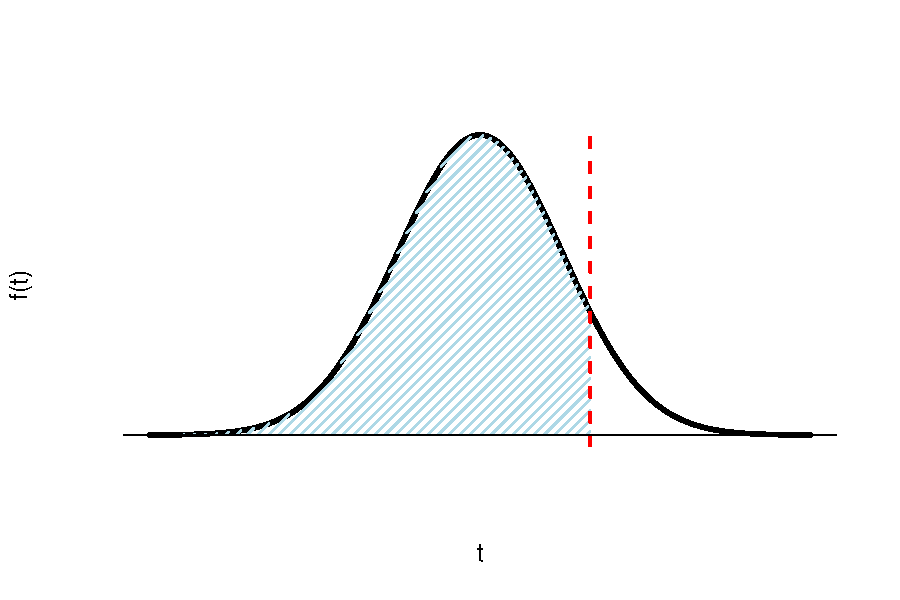
\includegraphics[width=\textwidth]{FIGS/L23-distrib_minf_b-1.pdf}
\end{minipage}
\end{frame}

\begin{frame}\frametitle{Survival function}
Another characterization of the distribution of the random variable $T$ is through the \defword{survival} (or \defword{sojourn}) function
\vfill
The survival function of state $A$ is given by 
\begin{equation}
  \S(t)=1-F(t)=\IP(T>t)
  \label{eq:survival}
\end{equation}
This gives a description of the \defword{sojourn time} of a
system in a particular state (the time spent in the state)
\vfill
$\S$ is a nonincreasing function (since $\S=1-F$
with $F$ a c.d.f.), and
$\S(0)=1$ (since $T$ is a nonnegative random variable)
\end{frame}



\maxFrameImage{FIGS/L23-pdf-cdf-surv-normal-1.pdf}

\begin{frame}
The \defword{average sojourn time} $\tau$ in state $A$ is given by
\[
\tau=E(T)=\int_0^\infty tf(t)dt
\]
Since $\lim_{t\to\infty}t\S(t)=0$, it follows that 
\[
\tau=\int_0^\infty \S(t)dt
\]
\vfill
\defword{Expected future lifetime}:
\[
\frac{1}{\S(t_0)} \int_0^{\infty} t\,f(t+t_0)\,dt 
\]
\vfill
\begin{eqnarray*}
\S(t)-\S(a)&=&\IP\left\{\textrm{survive during }
 (a,t)\textrm{ having survived until }a\right\} \\
&=& \exp\left(-\int_a^t h(u)du\right)
\end{eqnarray*}
\end{frame}

\begin{frame}\frametitle{Hazard rate}
The \defword{hazard rate} (or \defword{failure rate}) is
\begin{align*}
h(t) &= \lim_{\Delta t\to 0}\frac{\S(t)-\S(t+\Delta t)}{\Delta t} \\
& = \lim_{\Delta t\to 0} \frac{\IP(T<t+\Delta t | T\geq
t)}{\Delta t} \\
&= \frac{f(t)}{\S(t)}
\end{align*}
It gives probability of failure between $t$ and $\Delta t$, given survival to $t$.
\vfill
We have
\[
h(t)=-\frac{d}{dt}\ln\S(t)
\]
\end{frame}



\maxFrameImage{FIGS/L23-pdf-cdf-surv-hazard-normal-1.pdf}

%%%%%%%%%%%%%%%%%%%%%%%%%%%
\begin{frame}{Competing risks}
Suppose now that the system starts in state $A$ at time $t=0$ and that depending on which of the two events $\mathcal{E}_1$ or $\mathcal{E}_2$ takes place first, it switches to state $B_1$ or $B_2$, respectively
\vfill
Consider the random variables $T_A$, \emph{time spent} in state $A$ (or sojourn time in $A$), $T_{AB_1}$, \emph{time before switch to} $B_1$ and $T_{AB_2}$, \emph{time before switch to} $B_2$
\vfill
If we consider state $A$, we cannot observe the variables $T_{AB_1}$ or $T_{AB_2}$. What is observable is the sojourn time in $A$
\[
T^*_A=\min\left( T_{AB_1},T_{AB_2} \right)
\]
(where $^*$ indicates that a quantity is observable)
\end{frame}

\begin{frame}{Failure rate by type of event}
We have two (or more) types of events whose individual failure rates have to be accounted for
\begin{align*}
h_j(t) &= \lim_{\Delta t\to 0} \frac{\mathbb{P}( T<t+\Delta t, S=S_j | T\geq t)}{\Delta t} 
\end{align*}
where $\mathbb{P}(T<t+\Delta t, S=S_j | T\geq t)$ is the probability of failure due to cause $S_j$ ($j=1,2$ ici), i.e., $S$ is a discrete r.v. representing the event that is taking place
\end{frame}

\begin{frame}
By the law of total probability, since only one of the event can take place, if there are $n$ risks, then
$$
h(t) = \sum_{i=1}^n h_j(t)
$$
or, identically,
$$
\mathcal{S}(t)
=
\exp\left(
  -\int_0^t \sum\textstyle_{j=1}^n h_j(s)\ ds
\right)
$$
\end{frame}

\begin{frame}
As a consequence, suppose a process is subject to two competing exponential risks with respective distributions with parameters $\theta_1$ and $\theta_2$
\vfill
Then the mean sojourn time in the initial state before being affected by one of the two risks is
$$
\frac{1}{\theta_1+\theta_2}
$$
\end{frame}


%%%%%%%%%%%%%%%%%%%
%%%%%%%%%%%%%%%%%%%
%%%%%%%%%%%%%%%%%%%
%%%%%%%%%%%%%%%%%%%
\subsection{Two ``extreme'' distributions and a nicer one}
% The section page
\newSubSectionSlide{FIGS-slides-admin/Gemini_Generated_Image_5yvymh5yvymh5yvy.jpeg}

\begin{frame}\frametitle{The exponential distribution}
The random variable $T$ has an \defword{exponential} distribution if its
probability density function takes the form
\begin{equation}\label{eq:exp_distrib}
f(t)=\begin{cases}0&\textrm{if }t<0,\\
\theta e^{-\theta t}&\textrm{if }t\geq 0,
\end{cases}
\end{equation}
with $\theta>0$. Then the
survival function for state $A$ is of the form $\S(t)=e^{-\theta
  t}$, for $t\geq 0$, and the average sojourn time in state $A$ is
\[
\tau=\int_0^\infty e^{-\theta t}dt=\frac 1\theta
\]
\end{frame}

\begin{frame}\frametitle{Particularities of the exponential distribution}
The standard deviation of an exponential distribution is also $1/\theta$. When estimating $\theta$, it is impossible to distinguish the mean and the standard deviation
\vfill
The exponential distribution is \defword{memoryless}: its conditional probability obeys
\[
P(T > s + t\; |\; T > s) = P(T > t),\quad\forall s, t \ge 0
\]

The exponential and geometric distributions are the only memoryless probability distributions
\vfill
The exponential distribution has a constant hazard function $h(t)\equiv\theta$
\end{frame}



\maxFrameImage{FIGS/L23-pdf-cdf-surv-hazard-expon-1.pdf}

\begin{frame}\frametitle{The Dirac delta distribution}
If for some constant $\omega>0$,
\[
\S(t)=
\left\{
\begin{array}{ll}
1, & 0\leq t\leq\omega \\
0, & \omega<t
\end{array}
\right.
\]
meaning that $T$ has a Dirac delta distribution
$\delta_\omega(t)$, then the average sojourn time is
\[
\tau=\int_0^\omega dt=\omega
\]
with standard deviation $\sigma=0$
\end{frame}

\begin{frame}{The Gamma distribution}
R.v. $X$ is \defword{Gamma} distributed ($X\,\sim\Gamma(k, \theta)$) with \defword{shape parameter} $k$ and \defword{scale parameter} $\theta$ (or \defword{rate} $\beta = 1/\theta$) (all positive) if its probability density function takes the form
\begin{equation}\label{eq:gamma_distrib}
f(x;k,\theta) = \frac{x^{k-1} \mathrm{e}^{-\frac{x}{\theta}}}{\Gamma ( k)\theta ^k}
\end{equation}
where $x>0$ and $\Gamma$ is the Euler Gamma function, defined for all $z\in\mathbb{C}$ s.t. $\Re(z) > 0$ by
\[
\Gamma : z \mapsto \int_0^{+\infty}  t^{z-1}\,\mathrm{e}^{-t}\,\mathrm{d}t
\]
\end{frame}

\begin{frame}{Properties of the Gamma distribution}
Mean $k\theta$, variance $k\theta^2$
\vfill
Survival function
\[
\mathcal{S}(t)=
1-\frac{1}{\Gamma(k)}\gamma\left(
k,\frac{t}{\theta} 
\right)
=1-\frac{1}{\Gamma(k)}\gamma\left(
k,\beta t
\right)
\]
where 
\[
\gamma(a,x)=\int_0^x t^{a-1}{\rm e}^{-t}{\rm d}t
\]
is an incomplete Gamma function
\end{frame}



\maxFrameImage{FIGS/L23-pdf-cdf-surv-hazard-gamma-1.pdf}


%%%%%%%%%%%%%%%%%%%
%%%%%%%%%%%%%%%%%%%
%%%%%%%%%%%%%%%%%%%
%%%%%%%%%%%%%%%%%%%
\subsection{A simple cohort model with death} 
% The section page
\newSubSectionSlide{FIGS-slides-admin/Gemini_Generated_Image_5yvymh5yvymh5yvy.jpeg}

\begin{frame}\frametitle{A model for a cohort with one cause of death}
Consider a \defword{cohort} of individuals born at the same time, e.g., the same year
\vfill
\begin{itemize}
\item At time $t=0$, there are initially $N_0>0$ individuals
\item All causes of death are compounded together 
\item The time until death, for a given individual, is a random variable $T$, with continuous probability density distribution $f(t)$ and survival function $\S(t)$
\end{itemize}
\vfill
$N(t)$ the cohort population at time $t\geq 0$
\begin{equation}\label{eq:N_general}
N(t)=N_0\S(t)
\end{equation}
\vfill
$\S(t)$ proportion of initial population still alive at time $t$, so $N_0\S(t)$ number in the cohort still alive at time $t$
\end{frame}

\begin{frame}\frametitle{Case where $T$ is exponentially distributed}
Suppose that $T$ has an exponential distribution with mean $1/d$ (or parameter $d$), $f(t)=de^{-dt}$. Then the survival function is $\S(t)=e^{-dt}$, and \eqref{eq:N_general} takes the form
\begin{equation}\label{eq:N}
N(t)=N_0e^{-dt}
\end{equation}
\vfill
Now note that
\begin{align*}
\frac{d}{dt} N(t) &= -dN_0e^{-dt} \\
&= -dN(t)
\end{align*}
with $N(0)=N_0$.
\vfill
{\red $\Rightarrow$} The ODE $N'=-dN$ makes the assumption that the life expectancy at birth is exponentially distributed
\end{frame}



\begin{frame}
Survival function, $\S(t)=\IP(T>t)$, for an exponential distribution with mean 80 years
\begin{center}
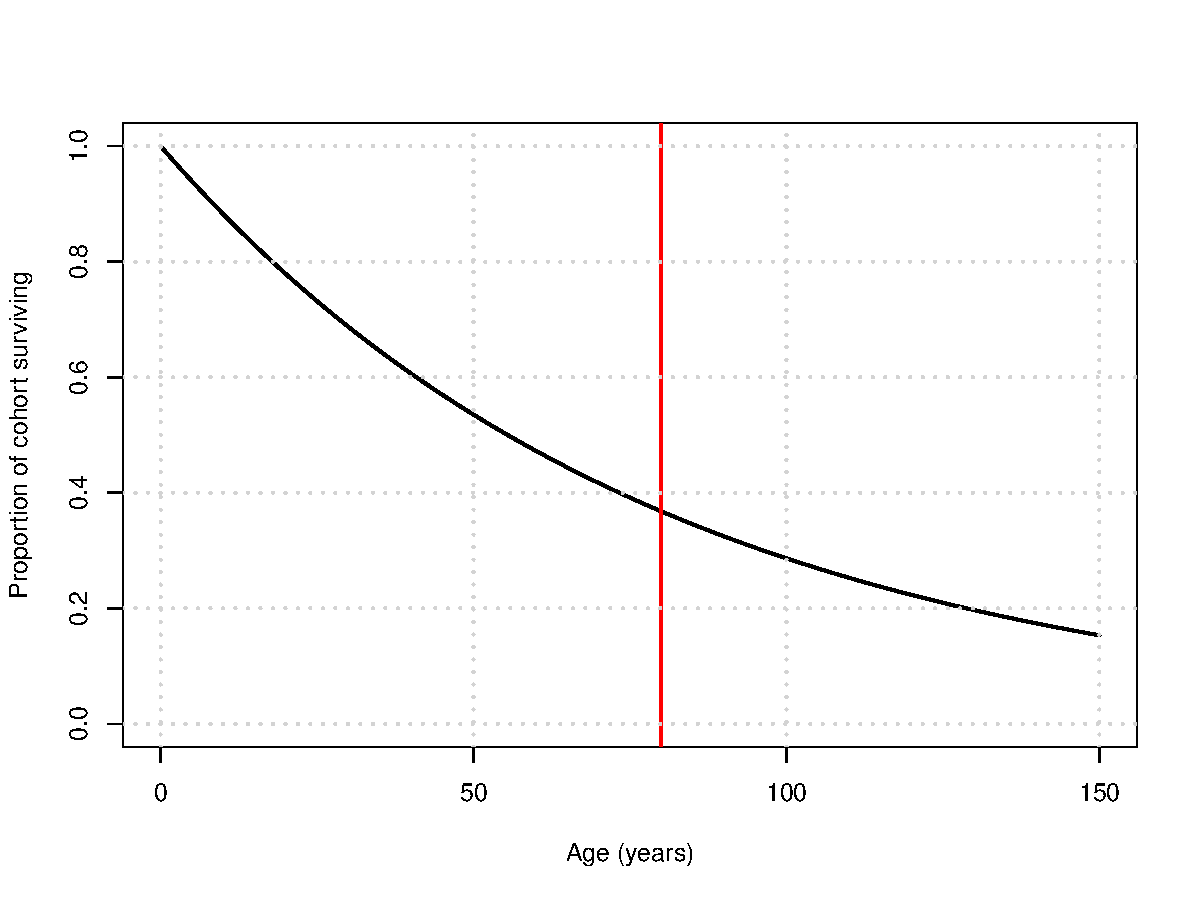
\includegraphics[width=0.8\textwidth]{FIGS/L23-prop_surviving_exp_80years-1.pdf}
\end{center}
\end{frame}


\begin{frame}\frametitle{Case where $T$ has a Dirac delta distribution}
Suppose that $T$ has a Dirac delta distribution at $t=\omega$, giving the
survival function 
\[
\S(t)=\begin{cases}
1, & 0\leq t\leq\omega \\
0, & t>\omega 
\end{cases}
\]
Then \eqref{eq:N_general} takes the form
\begin{equation}\label{eq:N2}
N(t)=\begin{cases}
N_0, & 0\leq t\leq\omega \\
0, & t>\omega
\end{cases}
\end{equation}
All individuals survive until time $\omega$, then they all die at time $\omega$
\vfill
Here, $N'=0$ everywhere except at $t=\omega$, where it is undefined
\end{frame}




\begin{frame}
Survival function, $\S(t)=\IP(T>t)$, for a Dirac distribution with mean 80 years
\begin{center}
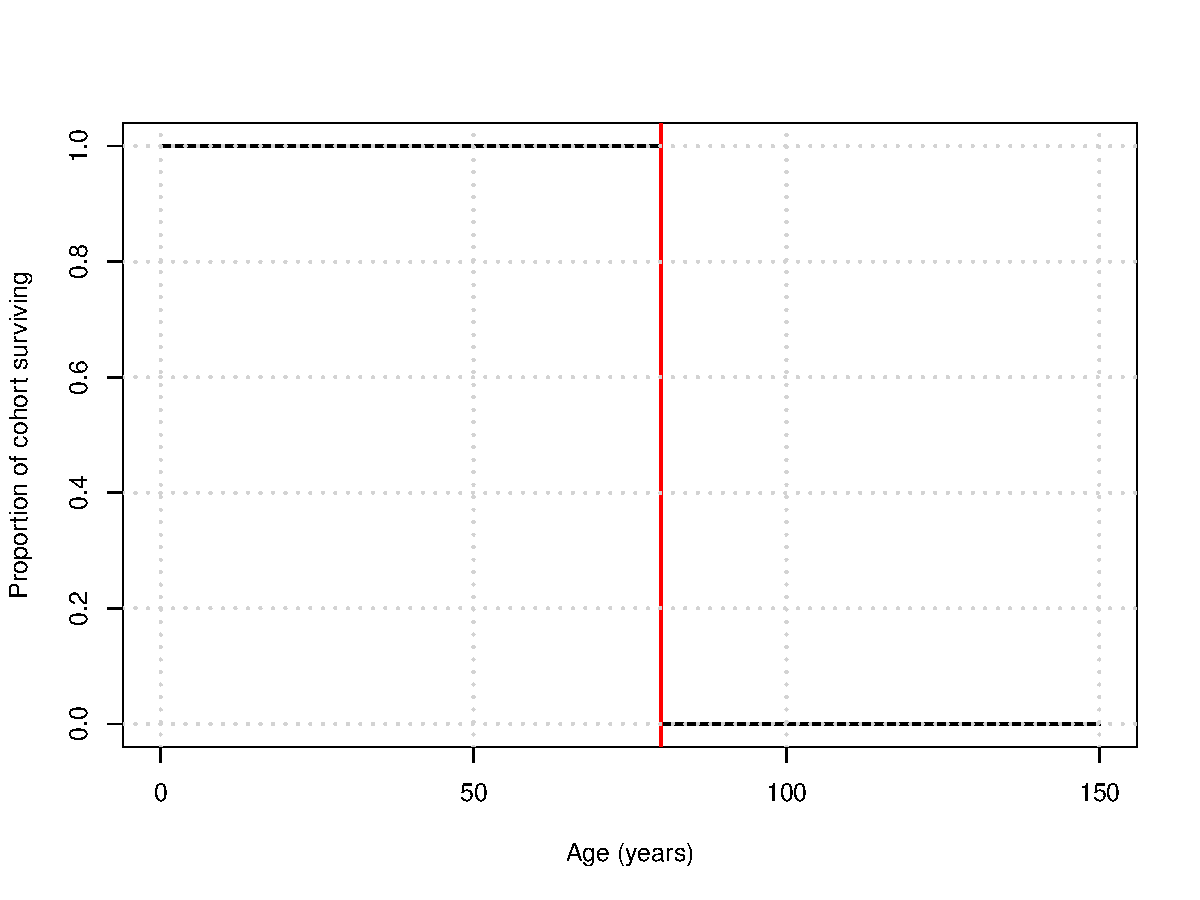
\includegraphics[width=0.8\textwidth]{FIGS/L23-prop_surviving_dirac_80years-1.pdf}
\end{center}
\end{frame}




%%%%%%%%%%%%%%%%%%%
%%%%%%%%%%%%%%%%%%%
%%%%%%%%%%%%%%%%%%%
%%%%%%%%%%%%%%%%%%%
\subsection{A possible fix to the exponential distribution issue} 
% The section page
\newSubSectionSlide{FIGS-slides-admin/Gemini_Generated_Image_5yvymh5yvymh5yvy.jpeg}



\begin{frame}{Survival for the exponential distribution}
\begin{center}
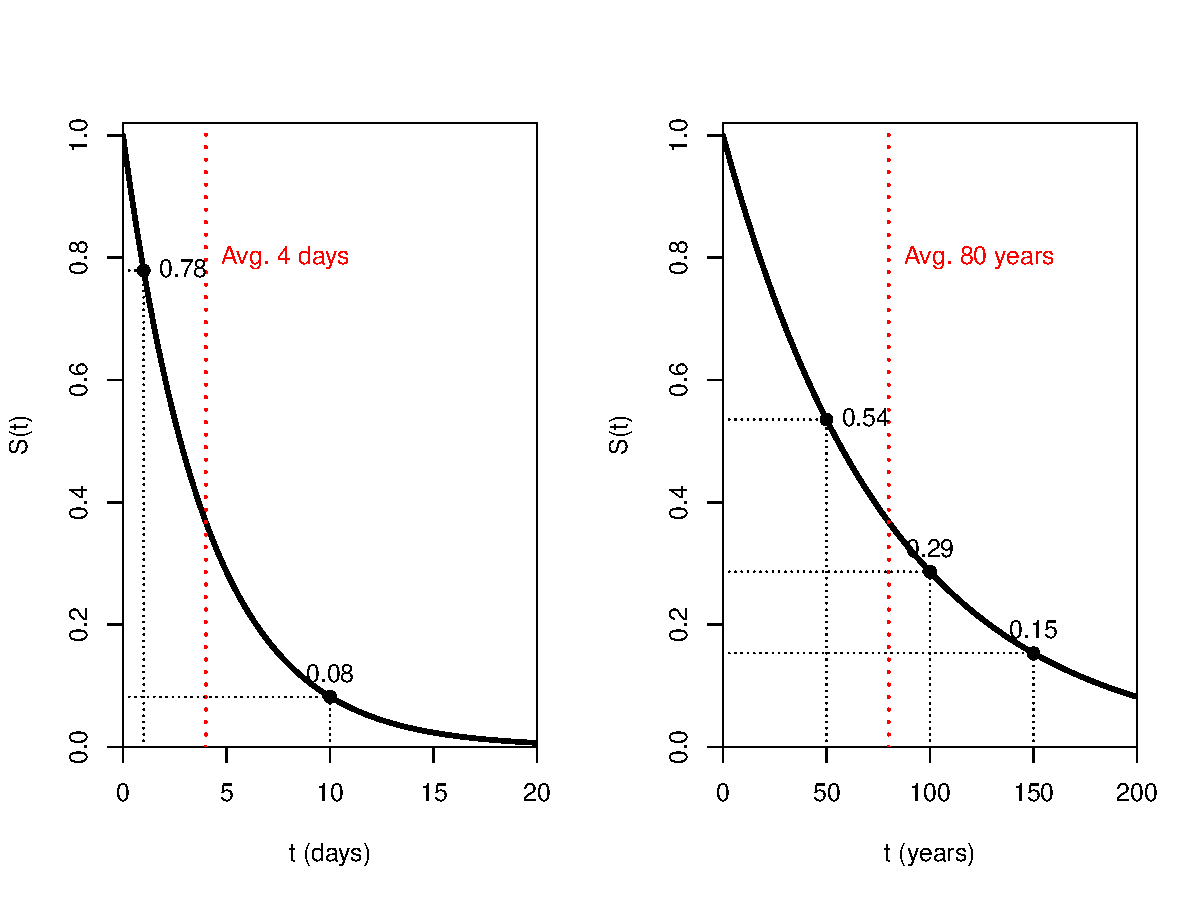
\includegraphics[width=0.75\textwidth]{FIGS/L23-prop_surviving_exp_80years_details-1.pdf}
\end{center}
\end{frame}

\begin{frame}{Issues with the exponential distribution}
\bbullet Survival drops quickly
\vfill
\bbullet Survival continues way beyond the mean
\vfill
Acceptable if what matters is the average duration of sojourn in a compartment (e.g., long term dynamics)
\vfill
More iffy if one is interested in short-term dynamics
\vfill
\bbullet Exponential distribution with parameter $\theta$ has same mean and standard deviation $1/\theta$, i.e., a single parameter controls mean and dispersion about the mean
\end{frame}

\begin{frame}{Exponential distributions are ``bad'' but also cool}
$X_1$ and $X_2$ 2 i.i.d. (independent and identically distributed) r.v. with parametres $\theta_1$ and $\theta_2$. Then the probability density function of the r.v. $Z=X_1+X_2$ is given by the convolution
\begin{align}
 f_Z(z) &= \int_{-\infty}^\infty f_{X_1}(x_1) f_{X_2}(z - x_1)\,dx_1 \nonumber\\
   &= \int_0^z \theta_1 e^{-\theta_1 x_1} \theta_2 e^{-\theta_2(z - x_1)} \, dx_1 \nonumber\\
   &= \theta_1 \theta_2 e^{-\theta_2 z} \int_0^z e^{(\theta_2 - \theta_1)x_1}\,dx_1 \nonumber\\
   &= \begin{cases}
        \dfrac{\theta_1 \theta_2}{\theta_2-\theta_1} \left(e^{-\theta_1 z} - e^{-\theta_2 z}\right) & \text{ if } \theta_1 \neq \theta_2 \\
        \theta^2 z e^{-\theta z} & \text{ if } \theta_1 = \theta_2 =: \theta
      \end{cases}
\end{align}
\end{frame}

\begin{frame}{The tool we use}
\begin{theorem}
Let $X_i$ be independent exponentially distributed random variables with parameter $\xi$ and $Y = \sum_{i=1}^n X_i$
\vskip1cm
Then the random variable $Y\rightsquigarrow E(n,\xi)$, an Erlang distribution with \emph{shape} parameter $n$ and \emph{scale} parameter $\xi$
\end{theorem}
\vfill
(Erlang distribution: Gamma distribution with integer shape parameter)
\end{frame}

\begin{frame}{Consequences for compartmental models}
If $n$ compartments are traversed successively by individuals, with each compartment having an outflow rate of $1/\xi$ (or a mean sojourn time of $\xi$), then the time of sojourn from entry into the first compartment to exit from the last is Erlang distributed with mean $E(Y)=n\xi$ and variance $\mathsf{Var}(Y)=n\xi^2$
\vfill
\begin{center}
\def\skip{*3}
\begin{tikzpicture}[scale=0.5, 
every node/.style={transform shape},
auto,
box/.style={minimum size=1.5cm, 
draw=black, very thick},
draw, circle]
%% States (imported original variants)
\node [box, fill=gray!20] at (0\skip,8) (X) {$X$};
\node [box, fill=gray!20] at (0\skip,4) (X1) {$X_{1}$};
\node [box, fill=gray!20] at (1\skip,4) (X2) {$X_{2}$};
\node [box, fill=gray!20] at (3\skip,4) (Xk) {$X_{k}$};
\node [box, fill=gray!20] at (5\skip,4) (XNm1) {$X_{N-1}$};
\node [box, fill=gray!20] at (6\skip,4) (XN) {$X_{N}$};
% Metabox
\draw [blue,rounded corners, thick, fill=blue!40, fill opacity=0.2] (-0.5\skip,9) -- (7\skip,9) -- (7\skip, 7) -- (-0.5\skip, 7) -- cycle;
\draw [blue,rounded corners, thick, fill=blue!40, fill opacity=0.2] (-0.5\skip,5) -- (7\skip,5) -- (7\skip, 3) -- (-0.5\skip, 3) -- cycle;
%% Flows (exponential box)
\path [line, very thick] (X) to node [midway, above] (TextNode) {$\mu X$} (7\skip,8);
%% Flows (Erlang box)
\path [line, very thick] (X1) to node [midway, above] (TextNode) {$\varepsilon X_1$} (X2);
\path [line, very thick] (X2) to node [midway, above] (TextNode) {$\varepsilon X_2$} (2\skip,4);
\path [line, very thick] (4\skip,4) to node [midway, above] (TextNode) {$\varepsilon X_{N-2}$} (XNm1);
\path [line, very thick] (XNm1) to node [midway, above] (TextNode) {$\varepsilon X_{N-1}$} (XN);
\path [line, very thick] (XN) to node [midway, above] (TextNode) {$\varepsilon X_{N}$} (7\skip,4);
%% To and from centre node
\path [line, very thick, dashed] (2.25\skip,4) to node [midway, above] (TextNode) {} (Xk);
\path [line, very thick, dashed] (Xk) to node [midway, above] (TextNode) {} (3.75\skip,4);
%% Time lines
\draw [|-|, thick] (0\skip,6.5) -- (7\skip,6.5);
\draw [|-|, thick] (0\skip,2.5) -- (7\skip,2.5);
%% Labels of time lines 
\node at (6\skip,2) {Average sojourn time $N/\varepsilon$};
\node at (6\skip,6) {Average sojourn time $1/\mu$};
\end{tikzpicture}
\end{center}
\vfill
I have a \href{https://daytah-or-dahtah.ovh:3838/Erlang_shiny/}{Shiny app} for this :)
\end{frame}

\begin{frame}{Example: EVD incubation periods}
Consider the incubation period for Ebola Virus Disease. During the 2014 EVD crisis in Western Africa, the WHO Ebola Response Team estimated incubation periods in a 2015 paper
\vfill
Table S2 in the Supplementary Information in that paper gives the best fit for the distribution of incubation periods for EVD as a Gamma distribution with mean 10.3 days and standard deviation 8.2, i.e., $n\varepsilon = 10.3$ and $\varepsilon \sqrt{n}=8.2$
\vfill
From this, $\varepsilon = 8.2^2/10.3 \simeq 6.53$ and $n = 10.3^2/8.2^2 \simeq 1.57$. However, that is a Gamma distribution
\end{frame}

\begin{frame}[fragile]{Switching to a compartmental model approach}
To use multiple compartments to better fit residence times, we need to find the closest possible Erlang distribution to this Gamma distribution
\vfill
$\implies$ compute RSS errors between data points generated from the given Gamma distribution and an Erlang
\vfill 
\begin{knitrout}
\definecolor{shadecolor}{rgb}{0.969, 0.969, 0.969}\color{fgcolor}\begin{kframe}
\begin{alltt}
\hldef{error_Gamma} \hlkwb{<-} \hlkwa{function}\hldef{(}\hlkwc{theta}\hldef{,}\hlkwc{shape}\hldef{,}\hlkwc{t}\hldef{,}\hlkwc{d}\hldef{) \{}
  \hldef{test_points} \hlkwb{<-} \hlkwd{dgamma}\hldef{(t,} \hlkwc{shape} \hldef{= shape,} \hlkwc{scale} \hldef{= theta)}
  \hldef{ls_error} \hlkwb{<-} \hlkwd{sum}\hldef{((d}\hlopt{-}\hldef{test_points)}\hlopt{^}\hlnum{2}\hldef{)}
  \hlkwd{return}\hldef{(ls_error)}
\hldef{\}}
\end{alltt}
\end{kframe}
\end{knitrout}

\end{frame}

\begin{frame}[fragile, allowframebreaks]

\begin{knitrout}
\definecolor{shadecolor}{rgb}{0.969, 0.969, 0.969}\color{fgcolor}\begin{kframe}
\begin{alltt}
\hldef{optimize_gamma} \hlkwb{<-} \hlkwa{function}\hldef{(}\hlkwc{t}\hldef{,}\hlkwc{d}\hldef{) \{}
  \hldef{max_shape} \hlkwb{<-} \hlnum{10}
  \hldef{error_vector} \hlkwb{<-} \hlkwd{mat.or.vec}\hldef{(max_shape,}\hlnum{1}\hldef{)}
  \hldef{scale_vector} \hlkwb{<-} \hlkwd{mat.or.vec}\hldef{(max_shape,}\hlnum{1}\hldef{)}
  \hlkwa{for} \hldef{(i} \hlkwa{in} \hlnum{1}\hlopt{:}\hldef{max_shape) \{}
    \hldef{result_optim} \hlkwb{<-} \hlkwd{try}\hldef{(}\hlkwd{optim}\hldef{(}\hlkwc{par} \hldef{=} \hlnum{3}\hldef{,}
                              \hlkwc{fn} \hldef{= error_Gamma,}
                              \hlkwc{lower} \hldef{=} \hlnum{0}\hldef{,}
                              \hlkwc{method} \hldef{=} \hlsng{"L-BFGS-B"}\hldef{,}
                              \hlkwc{shape} \hldef{= i,}
                              \hlkwc{t} \hldef{= t,}
                              \hlkwc{d} \hldef{= d),}
                        \hlnum{TRUE}\hldef{)}
    \hlkwa{if} \hldef{(}\hlopt{!}\hlkwd{inherits}\hldef{(result_optim,}\hlsng{"try-error"}\hldef{)) \{}
      \hldef{error_vector[i]} \hlkwb{<-} \hldef{result_optim}\hlopt{$}\hldef{value}
      \hldef{scale_vector[i]} \hlkwb{<-} \hldef{result_optim}\hlopt{$}\hldef{par}
    \hldef{\}} \hlkwa{else} \hldef{\{}
      \hldef{error_vector[i]} \hlkwb{<-} \hlnum{NaN}
      \hldef{scale_vector[i]} \hlkwb{<-} \hlnum{NaN}
    \hldef{\}}
  \hldef{\}}
  \hldef{result_optim} \hlkwb{<-} \hlkwd{data.frame}\hldef{(}\hlkwd{seq}\hldef{(}\hlnum{1}\hldef{,max_shape),}
                             \hldef{scale_vector,}
                             \hldef{error_vector)}
  \hlkwd{colnames}\hldef{(result_optim)} \hlkwb{<-} \hlkwd{c}\hldef{(}\hlsng{"shape"}\hldef{,}\hlsng{"scale"}\hldef{,}\hlsng{"error"}\hldef{)}
  \hldef{result_optim} \hlkwb{<-} \hldef{result_optim[}\hlkwd{complete.cases}\hldef{(result_optim),]}
  \hlkwd{return}\hldef{(result_optim)}
\hldef{\}}
\end{alltt}
\end{kframe}
\end{knitrout}

\end{frame}


\begin{frame}[fragile]

\begin{knitrout}
\definecolor{shadecolor}{rgb}{0.969, 0.969, 0.969}\color{fgcolor}\begin{kframe}
\begin{alltt}
\hldef{time_points} \hlkwb{<-} \hlkwd{seq}\hldef{(}\hlnum{0}\hldef{,}\hlnum{60}\hldef{)}
\hldef{data_points} \hlkwb{<-} \hlkwd{dgamma}\hldef{(time_points,} \hlkwc{shape} \hldef{=} \hlnum{1.57}\hldef{,}
                      \hlkwc{scale} \hldef{=} \hlnum{6.53}\hldef{)}
\hlcom{# Run the minimization}
\hldef{optim_fits} \hlkwb{<-} \hlkwd{optimize_gamma}\hldef{(time_points,data_points)}
\hlcom{# Which is the best Erlang to fit the data}
\hldef{idx_best} \hlkwb{<-} \hlkwd{which.min}\hldef{(optim_fits}\hlopt{$}\hldef{error)}
\end{alltt}
\end{kframe}
\end{knitrout}

\end{frame}



\begin{frame}
We find the best fit below, which is obtained using 2 compartments
\begin{center}
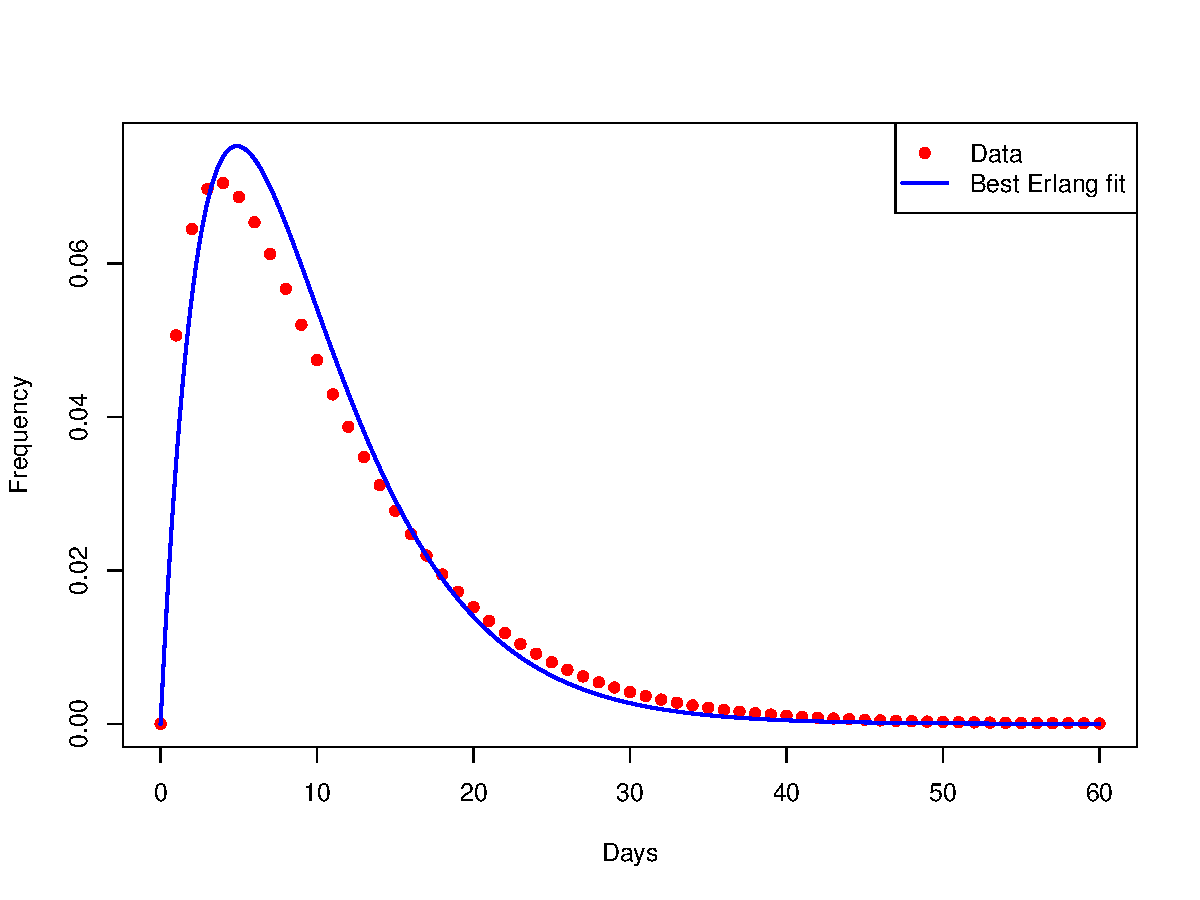
\includegraphics[width=0.75\textwidth]{FIGS/L23-plot_results_optim_Erlang-1.pdf}
\end{center}
\end{frame}






%%%%%%%%%%%%%%%%%%%
%%%%%%%%%%%%%%%%%%%
%%%%%%%%%%%%%%%%%%%
%%%%%%%%%%%%%%%%%%%
\subsection{Sojourn times in an SIS disease transmission model} 
% The section page
\newSubSectionSlide{FIGS-slides-admin/Gemini_Generated_Image_5yvymh5yvymh5yvy.jpeg}

\begin{frame}\frametitle{An SIS model}
\framesubtitle{Hypotheses}
\begin{itemize}
\item Individuals typically recover from the disease
\vfill
\item The disease does not confer immunity
\vfill
\item There is no birth or death (from the disease or natural) \newline\imply\;
Constant total population $N\equiv N(t)=S(t)+I(t)$
\vfill
\item Infection is of \defword{standard incidence} type
\end{itemize}
\end{frame}


\begin{frame}\frametitle{Recovery}
\begin{itemize}
\item Traditional models suppose that recovery occurs with rate constant
$\gamma$
\vfill
\item Here, of the individuals that become
infective at time $t_0$, a fraction $\S(t-t_0)$ remain infective at
time $t\geq t_0$
\vfill
\item \imply\;
For $t\geq 0$, $\S(t)$ is a survival function. As such, it verifies
$\S(0)=1$ and $\S$ is nonnegative and nonincreasing
\end{itemize}
\end{frame}


\begin{frame}\frametitle{Model for infectious individuals}
Since $N$ is constant, $S(t)=N-I(t)$ and we need only
consider the following equation (where $S$ is used for clarity)
\begin{equation}
I(t) = I_0(t)+ \int_0^t\beta\frac{S(u)I(u)}{N} \S(t-u) du
\label{eq:SIS_I} 
\end{equation}
\vfill
\begin{itemize}
\item $I_0(t)$ number of individuals who were infective at time
$t=0$ and still are at time $t$
\begin{itemize}
\item $I_0(t)$ is nonnegative, nonincreasing, and
such that $\lim_{t\to\infty}I_0(t)=0$
\end{itemize}
\item $\S(t-u)$ proportion of individuals who became infective at time $u$ and who still are at time $t$
\end{itemize}
\end{frame}


\begin{frame}\frametitle{Expression under the integral}
Integral equation for the number of infective individuals: 
\begin{equation}
I(t) = I_0(t)+ \int_0^t\beta\frac{(N-I(u))I(u)}{N} \S(t-u) du
\tag{\ref{eq:SIS_I}} 
\end{equation}
The term
\[
\beta\frac{(N-I(u))I(u)}{N} \S(t-u)
\]
\begin{itemize}
\item $\beta (N-I(u))I(u)/N$ is the rate at which new infectives are created, at time $u$
\item multiplying by $\S(t-u)$ gives the proportion of those who became
infectives at time $u$ and who still are at time $t$
\end{itemize}
Summing over $[0,t]$ gives the number of infective individuals at time $t$
\end{frame}


\begin{frame}\frametitle{Case of an exponentially distributed time to recovery}
Suppose $\S(t)$ such that sojourn time in the infective
state has exponential distribution with mean $1/\gamma$,
\textit{i.e.}, $\S(t)=e^{-\gamma t}$
\vfill
Initial condition function $I_0(t)$ takes the form
\[
I_0(t)=I_0(0)e^{-\gamma t}
\]
with $I_0(0)$ the number of infective individuals at time $t=0$. Obtained by considering the cohort of initially infectious individuals, giving a
model such as \eqref{eq:N_general}
\vfill
Equation (\ref{eq:SIS_I}) becomes
\begin{equation}\label{eq:I_ODE}
I(t)=I_0(0)e^{-\gamma t}+\int_0^t \beta\frac{(N-I(u))I(u)}{N} e^{-\gamma
(t-u)}du
\end{equation}
\end{frame}

\begin{frame}
Taking the time derivative of \eqref{eq:I_ODE} yields
\begin{align*}
I'(t) &= -\gamma I_0(0)e^{-\gamma t}-\gamma\int_0^t
\beta\frac{(N-I(u))I(u)}{N}e^{-\gamma(t-u)}du \\
&\quad +\beta \frac{(N-I(t))I(t)}{N} \\
&= -\gamma\left(I_0(0)e^{-\gamma t}+
\int_0^t \beta\frac{(N-I(u))I(u)}{N}e^{-\gamma(t-u)}du\right) \\
&\quad +\beta \frac{(N-I(t))I(t)}{N} \\
&= \beta \frac{(N-I(t))I(t)}{N}-\gamma I(t)
\end{align*}
\vfill
This is the classical logistic type ordinary differential equation (ODE) for $I$ in an SIS model without vital dynamics (no birth or death)
\end{frame}



\begin{frame}\frametitle{Case of a step function survival function}
Consider case where the time spent infected has survival function 
\[
\S(t)=\begin{cases}
1, & 0\leq t\leq\omega,\\
0, & t>\omega.
\end{cases}
\]
i.e., the sojourn time in the infective state is a constant
$\omega>0$
\vfill
In this case (\ref{eq:SIS_I}) becomes
\begin{equation}\label{eq:I_DDE}
I(t)=I_0(t)+\int_{t-\omega}^t \beta\frac{(N-I(u))I(u)}{N} du.
\end{equation}
Here, it is more difficult to obtain an expression for $I_0(t)$. It is however assumed that $I_0(t)$ vanishes for $t>\omega$
\end{frame}

\begin{frame}
When differentiated, \eqref{eq:I_DDE} gives, for $t\geq\omega$,
\[
I'(t)=I_0'(t)+\beta\frac{(N-I(t))I(t)}{N}
-\beta\frac{\left(N-I(t-\omega)\right)I(t-\omega)}{N}.
\]
Since $I_0(t)$ vanishes for $t>\omega$, this gives the delay
differential equation (DDE)
\[
I'(t)=\beta\frac{(N-I(t))I(t)}{N}
-\beta\frac{(N-I(t-\omega))I(t-\omega)}{N}.
\]
\end{frame}






%%%%%%%%%%%%%%%%%%%
%%%%%%%%%%%%%%%%%%%
\subsection{A model with vaccination}
% The section page
\newSubSectionSlide{FIGS-slides-admin/Gemini_Generated_Image_5yvymh5yvymh5yvy.jpeg}

\maxFrameImage{FIGS/ArinoCookePvdDVelasco.png}
\nocite{ArinoCookeVdDVelasco2004}

\begin{frame}\frametitle{Model structure}
\centering
\def\skip{*3.5}
\begin{tikzpicture}[scale=1, transform shape]
%% Regular nodes
\node [circle, fill=green!50, text=black] at (0,0) (S) {$S$};
\node [circle, fill=red!90, text=black] at (2\skip,0) (I) {$I$};
\node [circle, fill=blue!50, text=black] at (1\skip,-2) (V) {$V$};
%% Fake nodes for arrows
\node [left=2cm of S] (birthS) {};
\node [left=1.5cm of V] (birthV) {};
\node [above=0.75cm of S] (dS) {};
\node [above=0.75cm of I] (dI) {};
\node [below=0.75cm of V] (dV) {};
%% Flows
\path [line, very thick] (birthS) to node [midway, above] (TextNode) {$(1-\alpha)dN$} (S);
\path [line, very thick] (birthV) to node [midway, below] (TextNode) {$\alpha dN$} (V);
\path [line, very thick] (S) to node [midway, right] (TextNode) {$dS$} (dS);
\path [line, very thick] (I) to node [midway, right] (TextNode) {$dI$} (dI);
\path [line, very thick] (V) to node [midway, right] (TextNode) {$dV$} (dV);
\path [line, very thick, bend left=10] (S) to node [midway, above] (TextNode) {$\beta SI/N$} (I);
\path [line, very thick, bend left=10] (I) to node [midway, below] (TextNode) {$\gamma I$} (S);
\path [line, very thick, bend left=10] (S) to node [midway,above,sloped] (TextNode) {$\phi S$} (V);
\path [line, very thick, bend left=10,color=red] (V) to node [midway,below,sloped] (TextNode) {$\S(t)$} (S);
\path [line, very thick] (V) to node [midway, below, sloped] (TextNode) {$\sigma\beta VI/N$} (I);
\end{tikzpicture}    
\end{frame}

\begin{frame}\frametitle{Assumptions on $\S$}
$\S(t)$ is a nonnegative and nonincreasing function with $\S(0^+)=1$, and such that $\int_0^\infty \S(u)du$ is positive and finite
\vfill
So $\S(t)$ is a survival function
\end{frame}

\begin{frame}\frametitle{The SIS model with vaccination} 
\begin{subequations}\label{sys:SIVS_general}
\begin{align}
  \frac{dI(t)}{dt}&= \beta(S(t)+\sigma V(t))I(t)-(d+\gamma)I(t)
  \label{sys:SIVS_general_I}\\ 
  V(t)&= V_0(t)  
  +\int_0^t(\phi S(u)+\alpha d)\S(t-u)e^{-d(t-u)}
  e^{-\sigma\beta\int_u^tI(x)dx}du \label{sys:SIVS_general_V}
\end{align}
\end{subequations}
\vfill
\begin{itemize}
\item $\alpha d$ proportion of vaccinated newborns
\item $\phi S(u)$ proportion of vaccinated susceptibles
\item $\S(t-u)$ fraction of the proportion vaccinated still in the $V$
  class $t-u$ time units after going in
\item $e^{-d(t-u)}$ fraction of the proportion vaccinated
not dead due to natural causes
\item $e^{-\sigma\beta\int_u^t I(x)dx}$ fraction of the proportion
  vaccinated not gone to the infective class
\end{itemize} 
\end{frame}

\begin{frame}\frametitle{Reduction of the system using specific $\S(t)$ functions}
\vfill
\begin{itemize}
\item The distribution of waning times being exponential leads to
 an ODE system
\vfill
\item $\S(t)$ originating in a Dirac distribution leads to a discrete DDE model
\end{itemize}
\end{frame}


\begin{frame}{Be aware (beware?) of what's under the hood}
ODEs and discrete-delay DDEs are fine, but they hide some pretty strong assumptions
\vfill
If you are using an ODE for an \emph{endemic} model, fine: you are typically working with $t\to\infty$ and the ODE ``uses'' the mean of your parameter
\vfill
If, on the other hand, you are using an ODE to assess behaviour for times that are not too different from the mean of your parameters, then beware
\vfill
Discrete delays make the assumption that every single individual in your population has the same sojourn time if whatever compartment is being applied delay to... You may want to think about distributed delays or other mechanisms to compensate for this
\vfill
You may want to use a different hammer 
\end{frame}

%%%%%%%%%%%%%%%%%%%
%%%%%%%%%%%%%%%%%%%
%%%%%%%%%%%%%%%%%%%
%%%%%%%%%%%%%%%%%%%
\section{Continuous time Markov chains}
% The section page
\newSectionSlide{FIGS-slides-admin/Gemini_Generated_Image_bla659bla659bla6.jpeg}

\subsection{Continuous time Markov chains}
\newSubSectionSlide{FIGS-slides-admin/Gemini_Generated_Image_9agynl9agynl9agy.jpeg}
\begin{frame}
    \frametitle{From discrete to continuous time}
    \begin{block}{Discrete-Time Markov Chains (DTMCs)}
        A system transitions between states at fixed, discrete time steps ($n=0, 1, 2, \dots$)
        \begin{itemize}
            \item The future depends only on the present state (Markov Property)
            \item Governed by a \textbf{transition probability matrix} $P$, where $P_{ij}$ is the probability of moving from state $i$ to $j$ in one step
        \end{itemize}
    \end{block}
    
    \begin{block}{Continuous-Time Markov Chains (CTMCs)}
        A system can transition between states at \textbf{any point in time}
        \begin{itemize}
            \item Time spent in a state is a \textbf{continuous random variable}
            \item The ``holding time'' in any state $i$ follows an \textbf{exponential distribution} parameterised by an \textit{exit rate} $q_i$
            \item This is a direct consequence of the Markov Property being applied to continuous time (exponential is only continuous distribution that is ``memoryless'')
        \end{itemize}
    \end{block}
\end{frame}

\begin{frame}
    \frametitle{Transition rates}
    Dynamics of a CTMC defined by \textbf{transition rates}, not probabilities

    \begin{definition}[Transition Rates]
        For two states $i \neq j$, the rate $q_{ij} \ge 0$ is the instantaneous rate of transition from state $i$ to state $j$
        \begin{itemize}
            \item For a small time interval $\Delta t$, the probability of transitioning from $i$ to $j$ is approximately $q_{ij} \Delta t$
            \item Total \defword{exit rate} from state $i$ is $q_i = \sum_{j \neq i} q_{ij}$
            \item Time spent in state $i$ is an exponential random variable $T_i \sim \text{E}(q_i)$
        \end{itemize}
    \end{definition}
\end{frame}
    
\begin{frame}{The generator matrix}
    \begin{block}{Generator matrix (Q-Matrix)}
        Collect all transition rates into a single matrix $Q$
        \begin{itemize}
            \item Off-diagonal: $Q_{ij} = q_{ij}$ for $i \neq j$ (The rate of going from $i$ to $j$)
            \item Diagonal: $Q_{ii} = -q_i = -\sum_{j \neq i} q_{ij}$. (The negative of the total exit rate from $i$)
        \end{itemize}
        A key property is that all rows of $Q$ sum to zero: $\sum_{j} Q_{ij} = 0$.
    \end{block}
    
\end{frame}


\begin{frame}
    \frametitle{Kolmogorov equations}
    Let $P(t)$ be the matrix where $P_{ij}(t) = \mathbb{P}(X(t)=j | X(0)=i)$. How does $P(t)$ evolve over time?
    \vspace{1em}
    
    \begin{alertblock}{Kolmogorov forward equations}
        Describes rate of change of probability of ending up in a target state $j$
        $$ \frac{d}{dt}P(t) = P(t)Q $$
        In element form:
        $$ P'_{ij}(t) = \sum_{k} P_{ik}(t) Q_{kj} $$
    \end{alertblock}
\end{frame}

\begin{frame}{Solution to the KFE}
        The solution is the \textbf{matrix exponential}
        $$ P(t) = e^{tQ} = \sum_{k=0}^{\infty} \frac{(tQ)^k}{k!} $$
        \vfill
        The generator matrix $Q$ ``generates'' the process's evolution
\end{frame}


% \begin{frame}
%     \frametitle{The Stationary Distribution}
%     What happens to the process after a long time? Does it settle into an equilibrium?
%     
%     \begin{definition}[Stationary Distribution]
%         A probability distribution $\boldsymbol{\pi} = (\pi_1, \pi_2, \dots)$ is called a \textbf{stationary distribution} if, once the system is in this distribution, it stays in it.
%         $$ \boldsymbol{\pi} P(t) = \boldsymbol{\pi} \quad \text{for all } t \ge 0 $$
%         This implies that the distribution is no longer changing, i.e., $\frac{d}{dt}(\boldsymbol{\pi}P(t)) = \mathbf{0}$.
%     \end{definition}
%     
%     
%     \begin{block}{Finding the Stationary Distribution}
%         If a unique stationary distribution exists, it can be found by solving the system of linear equations:
%         $$ \boldsymbol{\pi} Q = \mathbf{0} $$
%         subject to the constraint that $\pi$ is a probability distribution:
%         $$ \sum_i \pi_i = 1 $$
%         The equation $\boldsymbol{\pi} Q = \mathbf{0}$ represents the "global balance" condition: for each state $j$, the total rate of probability flow into $j$ equals the total rate of probability flow out of $j$.
%     \end{block}
% \end{frame}



\subsection{ODE and CTMC}
% The section page
\newSubSectionSlide{FIGS-slides-admin/Gemini_Generated_Image_5yvymh5yvymh5yvy.jpeg}


\begin{frame}{Converting your compartmental ODE model to CTMC}
    Easy as $\pi$ :)
\vfill
\begin{itemize}
    \item Compartmental ODE model focuses on flows into and out of compartments
    \vfill
    \item ODE model has as many equations as there are compartments
    \vfill
    \item Compartmental CTMC model focuses on transitions
    \vfill
    \item CTMC model has as many transitions as there are arrows between (or into or out of) compartments
\end{itemize}
\end{frame}


\begin{frame}{ODE to CTMC : focus on different components}
    \begin{center}
        \begin{tikzpicture}[auto,
            scale=1.2, every node/.style={transform shape},
            cloud/.style={minimum width={width("N-1")+2pt},
            draw, ellipse,fill=red!20}]
            \node[cloud, fill=green!90, double=red] (S) at (0,0) {$S$};
            \node[cloud, draw=none, fill=white] (h4) at (2,0) {};
            \node[cloud, fill=red!90, double=red] (I) at (4,0) {$I$};
            \node[cloud, fill=green!90] (S2) at (6,0) {$S$};
            \node[cloud, fill=red!90] (I2) at (8,0) {$I$};
            %% Flows (ODE)
            \path [line, bend left, very thick, dashed] (S) to node [midway, above] (TextNode) {$-\beta SI$} (h4);
            \path [line, bend left, very thick] (h4) to node [midway, below] (TextNode) {$+\gamma I$} (S);
            \path [line, bend left, very thick] (h4) to node [midway, above] (TextNode) {$+\beta SI$} (I);
            \path [line, bend left, very thick, dashed] (I) to node [midway, below] (TextNode) {$-\gamma I$} (h4);
            %% Flows (CTMC)
            \path [line, bend left, very thick, red] (S2) to node [midway, above, black] (TextNode) {$\beta SI$} (I2);
            \path [line, bend left, very thick, red] (I2) to node [midway, below] (TextNode) {$\gamma I$} (S2);
            %%
            \draw[very thick, dotted] (5,-2) -- (5,2);
            %%
            \node[style=rectangle] at (2,2) {ODE};
            \node[style=rectangle] at (7,2) {CTMC};
            %%
            \node[style=rectangle] (fODE) at (2,-2) {focus};
            \path [line, dotted,red] (fODE) to  (S.south);
            \path [line, dotted,red] (fODE) to  (I.south);
            \node[style=rectangle] (fCTMC) at (6,-2) {focus};
            \path [line, dotted,red] (fCTMC) to (6.75,0.3);
            \path [line, dotted,red] (fCTMC) to  (6.75,-0.475);
        \end{tikzpicture}        
    \end{center}
\end{frame}


\begin{frame}{SIS without demography}
    \begin{center}
        \begin{tabular}{cp{3cm}cc}
          \toprule
            Transition & Effect & Weight & Probability \\
            \midrule
            $S\to S-1$, $I\to I+1$ & new infection & $\beta SI$ & $\dfrac{\beta SI}{\beta SI+\gamma I}$ \\
            $S\to S+1$, $I\to I-1$ & recovery of an infectious & $\gamma I$ & $\dfrac{\gamma I}{\beta SI+\gamma I}$ \\
            \bottomrule
        \end{tabular}
    \end{center}
    \vfill
    States are $S,I$
\end{frame}


\begin{frame}{SIS with demography}
    \begin{center}
        \begin{tabular}{p{3cm}p{3cm}cc}
        \toprule
            Transition & Effect & Weight & Probability \\
          \midrule
            $S\to S+1$ & birth of a susceptible & $b$ & $\frac{b}{b+d(S+I)+\beta SI+\gamma I}$ \\
            $S\to S-1$ & death of a susceptible & $dS$ & $\frac{dS}{b+d(S+I)+\beta SI+\gamma I}$ \\
            $S\to S-1$, $I\to I+1$ & new infection & $\beta SI$ & $\frac{\beta SI}{b+d(S+I)+\beta SI+\gamma I}$ \\
            $I\to I-1$ & death of an infectious & $dI$ & $\frac{dI}{b+d(S+I)+\beta SI+\gamma I}$ \\
            $S\to S+1$, $I\to I-1$ & recovery of an infectious & $\gamma I$ & $\frac{\gamma I}{b+d(S+I)+\beta SI+\gamma I}$ \\
            \bottomrule
        \end{tabular}
    \end{center}
\vfill
States are $S,I$
\end{frame}


\begin{frame}[fragile]{Kermack \& McKendrick model}
    \begin{center}
        \begin{tabular}{cp{3cm}cc}
        \toprule
            Transition & Effect & Weight & Probability \\
            \midrule
            $S\to S-1$, $I\to I+1$ & new infection & $\beta SI$ & $\dfrac{\beta SI}{\beta SI+\gamma I}$ \\
            $I\to I-1$, $R\to R+1$ & recovery of an infectious & $\gamma I$ & $\dfrac{\gamma I}{\beta SI+\gamma I}$ \\
            \bottomrule
        \end{tabular}
    \end{center}
    \vfill
    States are $S,I,R$
\end{frame}


\subsection{Simulating CTMC (in theory)}
% The section page
\newSubSectionSlide{FIGS-slides-admin/Gemini_Generated_Image_5yvymh5yvymh5yvy.jpeg}


\begin{frame}{Gillespie's algorithm}
    \begin{itemize}
        \item A.k.a. the stochastic simulation algorithm (SSA)
        \vfill
        \item Derived in 1976 by Daniel Gillespie
        \vfill
        \item Generates possible solutions for CTMC
        \vfill
        \item Extremely simple, so worth learning how to implement; there are however packages that you can use (see later)
    \end{itemize}
\end{frame}


\begin{frame}{Gillespie's algorithm}
Suppose system has state $\mathbf{x}(t)$ with initial condition $\mathbf{x}(t_0)=\mathbf{x}_0$ and \emph{propensity functions} $a_i$ of elementary reactions
\vfill
set $t\leftarrow t_0$ and $\mathbf{x}(t)\leftarrow \mathbf{x}_0$\\
while {$t\leq t_f$}\\
-\qquad $\xi_t\leftarrow \sum_j a_j(\mathbf{x}(t))$\\
-\qquad Draw $\tau_t$ from $T\thicksim \mathcal{E}(\xi_t)$\\
-\qquad Draw $\zeta_t$ from $\mathcal{U}([0,1])$\\
-\qquad Find $r$, smallest integer s.t. $\sum_{k=1}^j a_k(\mathbf{x}(t))> \zeta_t\sum_j a_j(\mathbf{x}(t))=\zeta_t\xi_t$\\
-\qquad Effect the next reaction (the one indexed $r$)\\
-\qquad $t\leftarrow t+\tau_t$\\    
\end{frame}


\begin{frame}{Drawing at random from an exponential distribution}
    If you do not have an exponential distribution random number generator.. We want $\tau_t$ from $T\thicksim\mathcal{E}(\xi_t)$, i.e., $T$ has probability density function
    $$
    f(x,\xi_t)=
    \xi_te^{-\xi_t x}\mathbf{1}_{x\geq 0}
    $$
    Use cumulative distribution function $F(x,\xi_t)=\int_{-\infty}^x f(s,\xi_t)\,ds$
    $$
    F(x,\xi_t)=
    (1-e^{-\xi_t x})\mathbf{1}_{x\geq 0}
    $$
    which has values in $[0,1]$. So draw $\zeta$ from $\mathcal{U}([0,1])$ and solve $F(x,\xi_t)=\zeta$ for $x$
    \begin{align*}
    F(x,\xi_t)=\zeta & \Leftrightarrow 1-e^{-\xi_tx}=\zeta \\
    &\Leftrightarrow e^{-\xi_tx} = 1-\zeta \\
    &\Leftrightarrow \xi_tx = -\ln(1-\zeta) \\
    &\Leftrightarrow \boxed{x = \frac{-\ln(1-\zeta)}{\xi_t}}
    \end{align*}
\end{frame}


\begin{frame}{Gillespie's algorithm (SIS model with only I eq.)}
set $t\leftarrow t_0$ and $I(t)\leftarrow I(t_0)$\\
while {$t\leq t_f$}\\
-\qquad $\xi_t\leftarrow \beta (P^\star-i)i+\gamma i$\\
-\qquad Draw $\tau_t$ from $T\thicksim \mathcal{E}(\xi_t)$\\
-\qquad $v\leftarrow\left[\beta (P^\star-i)i,\xi_t\right]/\xi_t$\\
-\qquad Draw $\zeta_t$ from $\mathcal{U}([0,1])$\\
-\qquad Find $pos$ such that $v_{pos-1}\leq\zeta_t\leq v_{pos}$\\
-\qquad switch {$pos$}\\
\qquad\qquad - 1: New infection, $I(t+\tau_t)=I(t)+1$ \\
\qquad\qquad - 2: End of infectious period, $I(t+\tau_t)=I(t)-1$ \\
- $t\leftarrow t+\tau_t$
\end{frame}


\begin{frame}{Sometimes Gillespie goes bad}
    \begin{itemize}
        \item Recall that the inter-event time is exponentially distributed
        \item Critical step of the Gillespie algorithm:
        \begin{itemize}
            \item $\xi_t\leftarrow$ weight of all possible events (\emph{propensity})
            \item Draw $\tau_t$ from $T\thicksim \mathcal{E}(\xi_t)$
        \end{itemize}
        \item So the inter-event time $\tau_t\to 0$ if $\xi_t$ becomes very large for some $t$
        \item This can cause the simulation to grind to a halt
    \end{itemize}
\end{frame}


\begin{frame}{Example: a birth and death process}
    \begin{itemize}
        \item Individuals born at \emph{per capita} rate $b$
        \item Individuals die at \emph{per capita} rate $d$
        \item Let's implement this using classic Gillespie
    \end{itemize}
    \vfill
(See \href{https://raw.githubusercontent.com/julien-arino/3MC-course-epidemiological-modelling/main/CODE/simulate_birth_death_CTMC.R}{\code{simulate\_birth\_death\_CTMC.R}} on course GitHub repo)
\end{frame}


\begin{frame}{Gillespie's algorithm (birth-death model)}
set $t\leftarrow t_0$ and $N(t)\leftarrow N(t_0)$\\
while {$t\leq t_f$}\\
-\qquad $\xi_t\leftarrow (b+d)N(t)$\\
-\qquad Draw $\tau_t$ from $T\thicksim \mathcal{E}(\xi_t)$\\
-\qquad $v\leftarrow\left[bN(t),\xi_t\right]/\xi_t$\\
-\qquad Draw $\zeta_t$ from $\mathcal{U}([0,1])$\\
-\qquad Find $pos$ such that $v_{pos-1}\leq\zeta_t\leq v_{pos}$\\
-\qquad switch {$pos$}\\
\qquad\qquad - 1: Birth, $N(t+\tau_t)=N(t)+1$ \\
\qquad\qquad - 2: Death, $N(t+\tau_t)=N(t)-1$ \\
- $t\leftarrow t+\tau_t$    
\end{frame}

\begin{frame}[fragile, allowframebreaks]

\begin{knitrout}
\definecolor{shadecolor}{rgb}{0.969, 0.969, 0.969}\color{fgcolor}\begin{kframe}
\begin{alltt}
\hldef{birth_death_CTMC} \hlkwb{=} \hlkwa{function}\hldef{(}\hlkwc{b} \hldef{=} \hlnum{0.01}\hldef{,} \hlkwc{d} \hldef{=} \hlnum{0.01}\hldef{) \{}
  \hldef{t_0} \hlkwb{=} \hlnum{0}    \hlcom{# Initial time}
  \hldef{N_0} \hlkwb{=} \hlnum{100}  \hlcom{# Initial population}

  \hlcom{# Vectors to store time and state. Initialise with initial condition.}
  \hldef{t} \hlkwb{=} \hldef{t_0}
  \hldef{N} \hlkwb{=} \hldef{N_0}

  \hldef{t_f} \hlkwb{=} \hlnum{1000}  \hlcom{# Final time}

  \hlcom{# Track the current time and state (could just check last entry in t}
  \hlcom{# and N, but will take more operations)}
  \hldef{t_curr} \hlkwb{=} \hldef{t_0}
  \hldef{N_curr} \hlkwb{=} \hldef{N_0}
  \hlkwa{while} \hldef{(t_curr}\hlopt{<=}\hldef{t_f) \{}
    \hldef{xi_t} \hlkwb{=} \hldef{(b}\hlopt{+}\hldef{d)}\hlopt{*}\hldef{N_curr}
    \hlkwa{if} \hldef{(N_curr} \hlopt{==} \hlnum{0}\hldef{) \{}
      \hlkwa{break} \hlcom{# Avoid error with rexp when xi_t = 0}
    \hldef{\}}
    \hldef{tau_t} \hlkwb{=} \hlkwd{rexp}\hldef{(}\hlnum{1}\hldef{,} \hlkwc{rate} \hldef{= xi_t)}
    \hldef{t_curr} \hlkwb{=} \hldef{t_curr}\hlopt{+}\hldef{tau_t}
    \hldef{v} \hlkwb{=} \hlkwd{c}\hldef{(b}\hlopt{*}\hldef{N_curr, xi_t)}\hlopt{/}\hldef{xi_t}
    \hldef{zeta_t} \hlkwb{=} \hlkwd{runif}\hldef{(}\hlkwc{n} \hldef{=} \hlnum{1}\hldef{)}
    \hldef{pos} \hlkwb{=} \hlkwd{findInterval}\hldef{(zeta_t, v)}\hlopt{+}\hlnum{1}
    \hlkwd{switch}\hldef{(pos,}
           \hldef{\{ N_curr} \hlkwb{=} \hldef{N_curr}\hlopt{+}\hlnum{1}\hldef{\},}  \hlcom{# Birth}
           \hldef{\{ N_curr} \hlkwb{=} \hldef{N_curr}\hlopt{-}\hlnum{1}\hldef{\})} \hlcom{# Death}
    \hldef{N} \hlkwb{=} \hlkwd{c}\hldef{(N, N_curr)}
    \hldef{t} \hlkwb{=} \hlkwd{c}\hldef{(t, t_curr)}
  \hldef{\}}
  \hlkwd{plot}\hldef{(t, N,} \hlkwc{type} \hldef{=} \hlsng{"l"}\hldef{,}
       \hlkwc{xlab} \hldef{=} \hlsng{"Time"}\hldef{,} \hlkwc{ylab} \hldef{=} \hlsng{"Population size"}\hldef{,}
       \hlkwc{main} \hldef{=} \hlkwd{paste}\hldef{(}\hlsng{"Birth-death CTMC with b ="}\hldef{, b,} \hlsng{"and d ="}\hldef{, d))}
\hldef{\}}
\end{alltt}
\end{kframe}
\end{knitrout}

\end{frame}



\maxFrameImage{FIGS/L23-CTMC_birth_death_b0_01_d0_01-1.pdf}



\maxFrameImage{FIGS/L23-CTMC_birth_death_b0_01_d0_02-1.pdf}

\begin{frame}[fragile]{$b=0.03$ \& $d=0.01$...}
We want to run the function with these parameter values but I know in advance this will not work well, so let's tweak the function a bit. We add a test:
\vfill
\begin{lstlisting}
if (t[length(t)]-t[(length(t)-1)] < 1e-8) {
      # If the time step is too small, stop the simulation
      message("Stopping simulation because time step is too small")
      break
    }
\end{lstlisting}
\vfill
\end{frame}





\maxFrameImage{FIGS/L23-CTMC_birth_death_b0_03_d0_01-1.pdf}




\begin{frame}[fragile]{Last one did not go well}
    \begin{itemize}
        \item Wanted 1000 time units (days?)
        \item Interrupted at 289.8661328 because of the test
        \newline (Slide with $b<d$: sim stopped because the population went extinct, I did not stop it!)
        \item At stop time
        \begin{itemize}
            \item $N =$ \ensuremath{4.2908\times 10^{4}}
            \item $|N| =$ 85961 (and $|t|$ as well, of course!)
            \item time was moving slowly
        \end{itemize}
    \end{itemize}
    \vfill
    
\begin{knitrout}
\definecolor{shadecolor}{rgb}{0.969, 0.969, 0.969}\color{fgcolor}\begin{kframe}
\begin{alltt}
\hlkwd{tail}\hldef{(}\hlkwd{diff}\hldef{(results}\hlopt{$}\hldef{t))}
\end{alltt}
\begin{verbatim}
## [1] 1.911574e-04 1.527582e-05 4.113673e-04 4.753229e-05 1.030327e-04
## [6] 6.899427e-09
\end{verbatim}
\end{kframe}
\end{knitrout}

\end{frame}


\maxFrameImage{FIGS/L23-plot_CTMC_birth_death_b0_03_d0_01_interevent-1.pdf}

\subsection{Simulating CTMC (in practice)}
% The section page
\newSubSectionSlide{FIGS-slides-admin/Gemini_Generated_Image_5yvymh5yvymh5yvy.jpeg}

\begin{frame}{Tau-leaping (and packages) to the rescue!}
    \begin{itemize}
        \item \emph{Approximation} method (compared to classic Gillespie, which is exact)
        \item Roughly: consider "groups" of events instead of individual events
        \item Good news: \code{GillespieSSA2} and \code{adaptivetau}, two standard packages for SSA in \code{R}, implement tau leaping
    \end{itemize}
\end{frame}

\begin{frame}[fragile, allowframebreaks]

\begin{knitrout}
\definecolor{shadecolor}{rgb}{0.969, 0.969, 0.969}\color{fgcolor}\begin{kframe}
\begin{alltt}
\hlkwd{library}\hldef{(GillespieSSA2)}
\hldef{Pop} \hlkwb{<-} \hlnum{1000}
\hldef{I_0} \hlkwb{<-} \hlnum{2}
\hldef{IC} \hlkwb{<-} \hlkwd{c}\hldef{(}\hlkwc{S} \hldef{= (Pop}\hlopt{-}\hldef{I_0),} \hlkwc{I} \hldef{= I_0)}
\hldef{gamma} \hlkwb{=} \hlnum{1}\hlopt{/}\hlnum{3}
\hlcom{# R0=beta/gamma*S0, so beta=R0*gamma/S0}
\hldef{beta} \hlkwb{=} \hlkwd{as.numeric}\hldef{(}\hlnum{1.5}\hlopt{*}\hldef{gamma}\hlopt{/}\hldef{IC[}\hlsng{"S"}\hldef{])}
\hldef{params} \hlkwb{<-} \hlkwd{c}\hldef{(}\hlkwc{gamma} \hldef{= gamma,} \hlkwc{beta} \hldef{= beta)}
\hldef{t_f} \hlkwb{=} \hlnum{100}
\hldef{reactions} \hlkwb{<-} \hlkwd{list}\hldef{(}
  \hlkwd{reaction}\hldef{(}\hlsng{"beta*S*I"}\hldef{,} \hlkwd{c}\hldef{(}\hlkwc{S}\hldef{=}\hlopt{-}\hlnum{1}\hldef{,}\hlkwc{I}\hldef{=}\hlopt{+}\hlnum{1}\hldef{),} \hlsng{"new_infection"}\hldef{),}
  \hlkwd{reaction}\hldef{(}\hlsng{"gamma*I"}\hldef{,} \hlkwd{c}\hldef{(}\hlkwc{S}\hldef{=}\hlopt{+}\hlnum{1}\hldef{,}\hlkwc{I}\hldef{=}\hlopt{-}\hlnum{1}\hldef{),} \hlsng{"recovery"}\hldef{)}
\hldef{)}
\hlkwd{set.seed}\hldef{(}\hlkwa{NULL}\hldef{)}


\hldef{sol} \hlkwb{<-} \hlkwd{ssa}\hldef{(}
  \hlkwc{initial_state} \hldef{= IC,}
  \hlkwc{reactions} \hldef{= reactions,}
  \hlkwc{params} \hldef{= params,}
  \hlkwc{method} \hldef{=} \hlkwd{ssa_exact}\hldef{(),}
  \hlkwc{final_time} \hldef{= t_f,}
\hldef{)}
\hlkwd{plot}\hldef{(sol}\hlopt{$}\hldef{time, sol}\hlopt{$}\hldef{state[,}\hlsng{"I"}\hldef{],} \hlkwc{type} \hldef{=} \hlsng{"l"}\hldef{,}
     \hlkwc{xlab} \hldef{=} \hlsng{"Time (days)"}\hldef{,} \hlkwc{ylab} \hldef{=} \hlsng{"Number infectious"}\hldef{)}
\end{alltt}
\end{kframe}
\end{knitrout}

\end{frame}

\maxFrameImage{FIGS/L23-sim-gillespie2-first-1.pdf}



\subsection{Parallelising your code in \code{R}}
% The section page
\newSubSectionSlide{FIGS-slides-admin/Gemini_Generated_Image_4oxcef4oxcef4oxc.jpeg}


\begin{frame}{Parallelisation}
    To see multiple realisations: good idea to parallelise, then interpolate results. Write a function, e.g.,  \code{run\_one\_sim} that .. runs one simulation
    \vfill
    Use some parallelisation mechanisms to run \code{run\_one\_sim} in parallel. One easy way to do it is to use a parallel version of \code{lapply}, which applies a function to a list
    \vfill
    Here, I am showing parallelisation using a recent-ish package called \code{future} (and \code{future.apply}, which contains the relevant \code{lapply} equivalent)
    \vfill
    I am also illustrating another SSA library that I find less tricky on Windows because the reactions are not precompiled: \code{adaptivetau}
\end{frame}

\begin{knitrout}
\definecolor{shadecolor}{rgb}{0.969, 0.969, 0.969}\color{fgcolor}\begin{kframe}
\begin{alltt}
\hlkwd{library}\hldef{(adaptivetau)}
\hlkwd{library}\hldef{(future.apply)}
\hlcom{# It is useful to have the transitions, rates and }
\hlcom{# names defined in a function}
\hldef{CTMC_SIS} \hlkwb{<-} \hlkwa{function}\hldef{() \{}
  \hlcom{# Define transitions for adaptivetau}
  \hldef{transitions} \hlkwb{<-} \hlkwd{list}\hldef{(}
    \hlkwd{c}\hldef{(}\hlkwc{S} \hldef{=} \hlopt{-}\hlnum{1}\hldef{,} \hlkwc{I} \hldef{=} \hlopt{+}\hlnum{1}\hldef{),}  \hlcom{# new_infection}
    \hlkwd{c}\hldef{(}\hlkwc{S} \hldef{=} \hlopt{+}\hlnum{1}\hldef{,} \hlkwc{I} \hldef{=} \hlopt{-}\hlnum{1}\hldef{)}   \hlcom{# recovery}
  \hldef{)}
  \hlcom{# Define rate function}
  \hldef{rates} \hlkwb{<-} \hlkwa{function}\hldef{(}\hlkwc{x}\hldef{,} \hlkwc{params}\hldef{,} \hlkwc{t}\hldef{) \{}
    \hlkwd{c}\hldef{(}
      \hldef{params[[}\hlsng{"beta"}\hldef{]]} \hlopt{*} \hldef{x[}\hlsng{"S"}\hldef{]} \hlopt{*} \hldef{x[}\hlsng{"I"}\hldef{],}
      \hldef{params[[}\hlsng{"gamma"}\hldef{]]} \hlopt{*} \hldef{x[}\hlsng{"I"}\hldef{]}
    \hldef{)}
  \hldef{\}}
  \hldef{event_names} \hlkwb{=} \hlkwd{c}\hldef{(}\hlsng{"new_infection"}\hldef{,} \hlsng{"recovery"}\hldef{)}
  \hlkwd{return}\hldef{(}\hlkwd{list}\hldef{(}\hlkwc{transitions} \hldef{= transitions,}
              \hlkwc{rates} \hldef{= rates,}
              \hlkwc{event_names} \hldef{= event_names))}
\hldef{\}}

\hldef{run_one_sim} \hlkwb{=} \hlkwa{function}\hldef{(}\hlkwc{CTMC}\hldef{,} \hlkwc{params}\hldef{) \{}
    \hldef{IC} \hlkwb{<-} \hlkwd{c}\hldef{(}\hlkwc{S} \hldef{= (params}\hlopt{$}\hldef{Pop}\hlopt{-}\hldef{params}\hlopt{$}\hldef{I_0),}
            \hlkwc{I} \hldef{= params}\hlopt{$}\hldef{I_0)}
    \hlkwd{set.seed}\hldef{(}\hlkwa{NULL}\hldef{)}
    \hldef{sol} \hlkwb{<-} \hlkwd{ssa.exact}\hldef{(}
        \hlkwc{init.values} \hldef{= IC,}
        \hlkwc{transitions} \hldef{= CTMC}\hlopt{$}\hldef{transitions,}
        \hlkwc{rateFunc} \hldef{= CTMC}\hlopt{$}\hldef{rates,}
        \hlkwc{params} \hldef{= params,}
        \hlkwc{tf} \hldef{= params}\hlopt{$}\hldef{t_f}
    \hldef{)}
    \hlcom{# Interpolate result (just I will do)}
    \hldef{wanted_t} \hlkwb{=}
      \hlkwd{seq}\hldef{(}\hlkwc{from} \hldef{=} \hlnum{0}\hldef{,} \hlkwc{to} \hldef{= params}\hlopt{$}\hldef{t_f,} \hlkwc{by} \hldef{=} \hlnum{0.01}\hldef{)}
    \hldef{interp_I} \hlkwb{=} \hlkwd{approx}\hldef{(}\hlkwc{x} \hldef{= sol[,}\hlsng{"time"}\hldef{],}
                      \hlkwc{y} \hldef{= sol[,}\hlsng{"I"}\hldef{],}
                      \hlkwc{xout} \hldef{= wanted_t)}
    \hlkwd{names}\hldef{(interp_I)} \hlkwb{=} \hlkwd{c}\hldef{(}\hlsng{"time"}\hldef{,} \hlsng{"I"}\hldef{)}
    \hldef{sol}\hlopt{$}\hldef{interp_I} \hlkwb{=} \hldef{interp_I}
    \hlcom{# Return result}
    \hlkwd{return}\hldef{(sol)}
\hldef{\}}

\hlcom{# By default, use all available cores}
\hlkwd{plan}\hldef{(multisession)}
\hlcom{## To use fewer workers, leaving one empty for }
\hlcom{# instance}
\hlcom{# plan(multisession, availableCores()-1)}
\hlcom{## To run sequentially}
\hlcom{# plan(sequential)}

\hlcom{# Set up parameters not needing computation}
\hldef{params} \hlkwb{<-} \hlkwd{list}\hldef{(}\hlkwc{gamma} \hldef{=} \hlnum{1}\hlopt{/}\hlnum{3}\hldef{,}
               \hlkwc{Pop} \hldef{=} \hlnum{1000}\hldef{,}
               \hlkwc{I_0} \hldef{=} \hlnum{2}\hldef{,}
               \hlkwc{R0} \hldef{=} \hlnum{1.5}\hldef{,}
               \hlkwc{t_f} \hldef{=} \hlnum{100}\hldef{,} \hlkwc{nb_sims} \hldef{=} \hlnum{50}\hldef{)}
\hldef{IC} \hlkwb{<-} \hlkwd{c}\hldef{(}\hlkwc{S} \hldef{= (params}\hlopt{$}\hldef{Pop}\hlopt{-}\hldef{params}\hlopt{$}\hldef{I_0),}
        \hlkwc{I} \hldef{= params}\hlopt{$}\hldef{I_0)}
\hlcom{# R0=beta/gamma*S0, so beta=R0*gamma/S0}
\hldef{params} \hlkwb{=}
  \hlkwd{c}\hldef{(params,}
    \hlkwc{beta} \hldef{=} \hlkwd{as.numeric}\hldef{(params}\hlopt{$}\hldef{R0}\hlopt{*}\hldef{params}\hlopt{$}\hldef{gamma} \hlopt{/}
                        \hldef{IC[}\hlsng{"S"}\hldef{]))}
\hlcom{# Run the simulation}
\hldef{CTMC} \hlkwb{<-} \hlkwd{CTMC_SIS}\hldef{()}
\hldef{SIMS} \hlkwb{=} \hlkwd{future_lapply}\hldef{(}
  \hlkwc{X} \hldef{=} \hlnum{1}\hlopt{:}\hldef{params}\hlopt{$}\hldef{nb_sims,}
  \hlkwc{FUN} \hldef{=}  \hlkwa{function}\hldef{(}\hlkwc{x}\hldef{)} \hlkwd{run_one_sim}\hldef{(CTMC, params))}
\hlcom{#  Liberate the workers!}
\hlkwd{stopCluster}\hldef{(cl)}
\end{alltt}


{\ttfamily\noindent\bfseries\color{errorcolor}{\#\# Error in stopCluster(cl): could not find function "{}stopCluster"{}}}\begin{alltt}
\hlcom{# Find max y value for plot}
\hldef{y_max} \hlkwb{=} \hlkwd{max}\hldef{(}\hlkwd{unlist}\hldef{(}\hlkwd{lapply}\hldef{(SIMS,} \hlkwa{function}\hldef{(}\hlkwc{x}\hldef{)} \hlkwd{max}\hldef{(x}\hlopt{$}\hldef{interp_I}\hlopt{$}\hldef{I))),}
            \hlkwc{na.rm} \hldef{=} \hlnum{TRUE}\hldef{)}
\hlcom{# Now plot}
\hlkwd{plot}\hldef{(SIMS[[}\hlnum{1}\hldef{]]}\hlopt{$}\hldef{interp_I}\hlopt{$}\hldef{time,}
     \hldef{SIMS[[}\hlnum{1}\hldef{]]}\hlopt{$}\hldef{interp_I}\hlopt{$}\hldef{I,}
     \hlkwc{type} \hldef{=} \hlsng{"l"}\hldef{,} \hlkwc{lwd} \hldef{=} \hlnum{0.5}\hldef{,}
     \hlkwc{xlab} \hldef{=} \hlsng{"Time (days)"}\hldef{,}
     \hlkwc{ylab} \hldef{=} \hlsng{"Number infectious"}\hldef{,}
     \hlkwc{ylim} \hldef{=} \hlkwd{c}\hldef{(}\hlnum{0}\hldef{, y_max),}
     \hlkwc{main} \hldef{=} \hlkwd{paste}\hldef{(}\hlsng{"CTMC with R0 ="}\hldef{, params}\hlopt{$}\hldef{R0))}
\hlkwa{for} \hldef{(i} \hlkwa{in} \hlnum{2}\hlopt{:}\hlkwd{length}\hldef{(SIMS)) \{}
  \hlkwd{lines}\hldef{(SIMS[[i]]}\hlopt{$}\hldef{interp_I}\hlopt{$}\hldef{time,}
        \hldef{SIMS[[i]]}\hlopt{$}\hldef{interp_I}\hlopt{$}\hldef{I,}
        \hlkwc{type} \hldef{=} \hlsng{"l"}\hldef{,} \hlkwc{lwd} \hldef{=} \hlnum{0.5}\hldef{)}
\hldef{\}}
\end{alltt}
\end{kframe}
\end{knitrout}

\begin{frame}[fragile, allowframebreaks]{Common part -- The function we run}

\begin{knitrout}
\definecolor{shadecolor}{rgb}{0.969, 0.969, 0.969}\color{fgcolor}\begin{kframe}
\begin{alltt}
\hldef{run_one_sim} \hlkwb{=} \hlkwa{function}\hldef{(}\hlkwc{params}\hldef{) \{}
    \hldef{IC} \hlkwb{<-} \hlkwd{c}\hldef{(}\hlkwc{S} \hldef{= (params}\hlopt{$}\hldef{Pop}\hlopt{-}\hldef{params}\hlopt{$}\hldef{I_0),} \hlkwc{I} \hldef{= params}\hlopt{$}\hldef{I_0)}
    \hldef{params_local} \hlkwb{<-} \hlkwd{c}\hldef{(}\hlkwc{gamma} \hldef{= params}\hlopt{$}\hldef{gamma,} \hlkwc{beta} \hldef{= params}\hlopt{$}\hldef{beta)}
    \hldef{reactions} \hlkwb{<-} \hlkwd{list}\hldef{(}
        \hlcom{# propensity function effects name for reaction}
        \hlkwd{reaction}\hldef{(}\hlsng{"beta*S*I"}\hldef{,} \hlkwd{c}\hldef{(}\hlkwc{S}\hldef{=}\hlopt{-}\hlnum{1}\hldef{,}\hlkwc{I}\hldef{=}\hlopt{+}\hlnum{1}\hldef{),} \hlsng{"new_infection"}\hldef{),}
        \hlkwd{reaction}\hldef{(}\hlsng{"gamma*I"}\hldef{,} \hlkwd{c}\hldef{(}\hlkwc{S}\hldef{=}\hlopt{+}\hlnum{1}\hldef{,}\hlkwc{I}\hldef{=}\hlopt{-}\hlnum{1}\hldef{),} \hlsng{"recovery"}\hldef{)}
    \hldef{)}
    \hlkwd{set.seed}\hldef{(}\hlkwa{NULL}\hldef{)}
    \hldef{sol} \hlkwb{<-} \hlkwd{ssa}\hldef{(}
      \hlkwc{initial_state} \hldef{= IC,}
      \hlkwc{reactions} \hldef{= reactions,}
      \hlkwc{params} \hldef{= params_local,}
      \hlkwc{method} \hldef{=} \hlkwd{ssa_exact}\hldef{(),}
      \hlkwc{final_time} \hldef{= params}\hlopt{$}\hldef{t_f,}
      \hlkwc{log_firings} \hldef{=} \hlnum{TRUE}    \hlcom{# This way we keep track of events}
    \hldef{)}
    \hlcom{# Interpolate result (just I will do)}
    \hldef{wanted_t} \hlkwb{=} \hlkwd{seq}\hldef{(}\hlkwc{from} \hldef{=} \hlnum{0}\hldef{,} \hlkwc{to} \hldef{= params}\hlopt{$}\hldef{t_f,} \hlkwc{by} \hldef{=} \hlnum{0.01}\hldef{)}
    \hldef{sol}\hlopt{$}\hldef{interp_I} \hlkwb{=} \hlkwd{approx}\hldef{(}\hlkwc{x} \hldef{= sol}\hlopt{$}\hldef{time,} \hlkwc{y} \hldef{= sol}\hlopt{$}\hldef{state[,}\hlsng{"I"}\hldef{],}
                          \hlkwc{xout} \hldef{= wanted_t)}
    \hlkwd{names}\hldef{(sol}\hlopt{$}\hldef{interp_I)} \hlkwb{=} \hlkwd{c}\hldef{(}\hlsng{"time"}\hldef{,} \hlsng{"I"}\hldef{)}
    \hlcom{# Return result}
    \hlkwd{return}\hldef{(sol)}
\hldef{\}}
\end{alltt}
\end{kframe}
\end{knitrout}

\end{frame}

\begin{frame}[fragile, allowframebreaks]

\end{frame}

\maxFrameImage{FIGS/L23-parallel-CTMC-plot-1.pdf}

\begin{frame}[fragile]{Benefit of parallelisation}
    Run the parallel code for 100 sims between `tictoc::tic()` and `tictoc::toc()`, giving `66.958 sec elapsed`, then the sequential version
\begin{lstlisting}
tictoc::tic()
SIMS = lapply(X = 1:params$number_sims,
                FUN =  function(x) run_one_sim(params))
tictoc::toc()
\end{lstlisting}
    which gives `318.141 sec elapsed` on a 6C/12T Intel(R) Core(TM) i9-8950HK CPU @ 2.90GHz (4.75$\times$ faster) or `12.067 sec elapsed` versus `258.985 sec elapsed` on a 32C/64T AMD Ryzen Threadripper 3970X 32-Core Processor (21.46$\times$ faster !)
\end{frame}


\subsection{Example -- Stochastic phase of an epidemic}
% The section page
\newSubSectionSlide{FIGS-slides-admin/Gemini_Generated_Image_5yvymh5yvymh5yvy.jpeg}

\maxFrameImage{FIGS/ArinoMilliken-BMB}
\nocite{ArinoMilliken2022b}

\maxFrameImage{FIGS/select_Wyoming-Campbell_bars_zoom}

\begin{frame}{Investigating outbreak types using a simple CTMC SIS}
\[
\mathbf{X}(t)=\left(S^A(t),I^A(t)\right)
\]
\vfill
CTMC $\mathbf{X}(t)$ characterized by transitions
\begin{center}
  \begin{tabular}{ccc}
    \toprule
    Description & Transition & Rate \\
    \midrule
    Infection & $\left(S^A,I^A\right)\to \left(S^A-1,I^A+1\right)$ & $\beta^AS^AI^A$ \\
    Recovery & $\left(S^A,I^A\right)\to \left(S^A+1,I^A-1\right)$ & $\gamma^AI^A$ \\
    \bottomrule
  \end{tabular}
\end{center}
\end{frame}

\begin{frame}{Investigating outbreak types using a simple CTMC SIS \emph{with a twist}}
Regular chain of this type has $I=0$ as sole absorbing state
\vfill
We add another absorbing state: if $I=\hat I$, then the chain has \emph{left} the stochastic phase and is in a quasi-deterministic phase with exponential growth
\vfill
Doing this, time to absorption measures become usable additionally to first passage time ones
\vfill
And the question becomes: how long does the chain ``linger on'' (``stutter'') before it is absorbed? We define the inter-absorption trajectory as the stochastic phase
\end{frame}

\maxFrameImage{FIGS/illustration_stochastic_phase.png}
\maxFrameImage{FIGS/duration_stochastic_phase_1patch_pop1M_I0eq1.png}

\begin{frame}{Problem of the value of the upper bound $\hat I$}
  \begin{itemize}
    \item Choose $\hat I$ too small and the stochastic phase will not last long
    \vfill
    \item Choose $\hat I$ too large and absorption will only be at the DFE
    \vfill
    \item So, how does one choose $\hat I$ ?
    \begin{itemize}
      \item A formula of Whittle (1955) \nocite{whittle1955}
      \item Multitype branching process (MTBP)
    \end{itemize}
  \end{itemize}
\end{frame}

%%%%%%%%%%%%%%%%%%%
%%%%%%%%%%%%%%%%%%%
%%%%%%%%%%%%%%%%%%%
%%%%%%%%%%%%%%%%%%%
\subsection{Value of travel control measures}
% The section page
\newSubSectionSlide{FIGS-slides-admin/Gemini_Generated_Image_bla65bbla65bbla6.jpeg}

\begin{frame}{}
  \centering
  \def\hstep{*3}
  \begin{tikzpicture}[scale=0.75, rotate=270,
    every node/.style={transform shape},
    auto,
    box/.style={minimum width={width("N-1")+2pt},
      draw, rectangle}]
    % Exporter
    \node [box] at (0\hstep,3) (SE) {$S_E$};
    \node [box] at (1\hstep,3) (LE) {$L_E$};
    \node [box] at (2\hstep,4.5) (DE) {$D_E$};
    \node [box] at (2\hstep,1.5) (UE) {$U_E$};
    \node [box] at (3\hstep,3) (RE) {$R_E$};
    %% Introduction layer
    % \node [box] at (0\hstep,9) (SI) {$S_I$};
    \node [box, fill=blue!50] at (1\hstep,9) (LI) {$L_{I}$};
    \node [box, fill=red!50] at (2\hstep,7.5) (DI) {$D_{I}$};
    \node [box, fill=blue!50] at (2\hstep,10.5) (UI) {$U_{I}$};
    %\node [box, fill=red!50] at (3\hstep,7.5) (RID) {$R_{ID}$};
    %% Community
    \node [box] at (0\hstep,13.5) (SC) {$S_C$};
    \node [box] at (1\hstep,13.5) (LC) {$L_{C}$};
    \node [box] at (2\hstep,15) (DC) {$D_{C}$};
    \node [box] at (2\hstep,12) (UXC) {$U_{C}$};
    \node [box] at (3\hstep,13.5) (RC) {$R_{C}$};
    %\node [box] at (3\hstep,12) (RCU) {$R_{CU}$};
    % Text
    \node[rotate=90] at (-1,2.5) {\Large\textbf{Exporter}};
    \node[rotate=90] at (-1,11.25) {\Large\textbf{Importer}};
    % "meta-boxes" around sets of compartments
    \draw [black,rounded corners] (-0.65,1) -- (-0.65,5) -- (3\hstep+0.7,5) -- (3\hstep+0.7,1) -- cycle;
    \draw [black,rounded corners] (-0.65,6.9) -- (-0.65,16) -- (3\hstep+0.7,16) -- (3\hstep+0.7,6.9) -- cycle;
    \draw [black,rounded corners, dotted] (-0.55,11.25) -- (3\hstep+0.6,11.25) -- (3\hstep+0.6,7.05) -- (-0.55,7.05)  -- cycle node at (2.75, 11) {\textbf{Introduction layer}};
    \draw [black,rounded corners, dotted] (-0.55,11.25) -- (3\hstep+0.6,11.25) -- (3\hstep+0.6,15.9) -- (-0.55,15.9)  -- cycle node at (2.2, 11.5) {\textbf{Community}};
    %% Flows in exporter
    \path [line,thick] (SE) to node [above, sloped] (TextNode) {$\Phi_E S_E$} (LE);
    \path [line,thick] (LE) to node [midway,above,sloped] (TextNode) {$p_E\varepsilon_E L_E$} (DE);
    \path [line,thick] (LE) to node [midway,above,sloped] (TextNode) {$(1-p_E)\varepsilon_E L_E$} (UE);
    \path [line,thick] (UE) to node [midway,above,sloped] (TextNode) {$(1-\delta_E)\gamma_E U_E$} (RE);
    \path [line,thick] (DE) to node [midway,above,sloped] (TextNode) {$(1-\delta_E)\gamma_E D_E$}  (RE);
    %\path [line, very thick] (DE) to node [pos=0.15, right=0.25cm] (TextNode) {$(1-\delta_E)\gamma_E D_E$}  (RE);
    %% Flows from exporter to importer
    \path [line,sloped] (SE) to node [pos=0.275, above] (TextNode) {$m_{S} S_E$} (SC);
    \path [line,dashed] (LE) to node [midway, above, sloped, rotate=180] (TextNode) {$m_L L_E$} (LI);
    \path [line,dashed] (DE) to node [midway, above, sloped, rotate=180] (TextNode) {$m_D D_E$} (DI);
    \path [line,dashed, bend right=20] (UE) to node [midway, above, sloped, rotate=180] (TextNode) {$m_U U_E$} (UI);
    %\path [line, thin, bend right=20] (RE) to node [midway, below, sloped] (TextNode) {$m_{R} R_E$} (RCU);
    \draw[-{Stealth}] (RE) -- (3\hstep+1,3) -- (3\hstep+1,13.5)  node [pos=0.29, above, sloped] (TextNode) {$m_{R} R_E$} -- (RC);
    %% Flows (introduction layer)
    % \path [line, very thick] (SI) to node [above, sloped] (TextNode) {$\Phi_I S_I$} (LI);
    \path [line,thick] (LI) to node [midway,below,sloped] (TextNode) {$p_{I}\varepsilon_I L_{I}$} (DI);
    \path [line,thick] (LI) to node [midway,above,sloped] (TextNode) {$(1-p_{I})\varepsilon_I L_{I}$} (UI);
    \path [line,thick] (DI) -- (3\hstep,7.5) -- node [midway, above,sloped] (TextNode) {$(1-\delta_I)\gamma_I D_{I}$} (RC);
    \path [line,thick] (UI) to node [midway,below,sloped] (TextNode) {$(1-\delta_I)\gamma_I U_{I}$} (RC);
    %% Flows (community)
    \path [line,thick] (SC) to node [midway, above, sloped] (TextNode) {$\Phi_C S_C$} (LC);
    \path [line,thick] (LC) to node [midway, above, sloped] (TextNode) {$p_C\varepsilon_C L_C$} (DC);
    \path [line,thick] (LC) to node [midway,above,sloped] (TextNode) {$(1-p_C)\varepsilon_C L_{C}$} (UXC);
    \path [line,thick] (DC) to node [midway, above,sloped] (TextNode) {$(1-\delta_C)\gamma_C D_{C}$} (RC);
    \path [line,thick] (UXC) to node [midway, above,sloped] (TextNode) {$(1-\delta_C)\gamma_C U_{C}$} (RC);
  \end{tikzpicture}		
\end{frame}

\maxFrameImage{FIGS/sim_2023_07_11-11_06_41_ID_9_run86.png}
\maxFrameImage{FIGS/sim_2023_07_11-11_06_41_ID_9_run2.png}
\maxFrameImage{FIGS/sim_2023_07_11-11_06_41_ID_9_run3.png}
\maxFrameImage{FIGS/sim_2023_07_11-11_06_41_ID_25_run5.png}
\maxFrameImage{FIGS/exporter_importer_panel_zoom.png}

\begin{frame}{One last thought for the road}
  V. Chetail. \href{https://doi.org/10.3389/fpos.2020.606307}{Crisis without borders: What does international law say about border closure in the context of Covid-19?} Frontiers in Political Science, 2 (12) (2020) \nocite{chetail2020crisis}
  \vfill
  \begin{quote}
    [..] a powerful expression of state's sovereignty, immigration control provides a typical avenue for governments to reassure their citizens and bolster a national sense of belonging, while providing an ideal scapegoat for their own failure or negligence.
  \end{quote}
\end{frame}



%%%%%%%%%%%%%%%%%%%
%%%%%%%%%%%%%%%%%%%
%%%%%%%%%%%%%%%%%%%
%%%%%%%%%%%%%%%%%%%
\section{Branching process approximations of CTMC}
% The section page
\newSectionSlide{FIGS-slides-admin/Gemini_Generated_Image_5yvymh5yvymh5yvy.jpeg}

\begin{frame}
    \frametitle{What is a Branching Process?}
    \begin{block}{The Core Idea}
        A branching process is a mathematical model for a population where individuals produce a random number of offspring and then die.
    \end{block}
    
    \begin{itemize}
        \item Think of bacteria splitting, a virus spreading, or even the survival of family surnames.
        \item We start with an initial population, $Z_0$.
        \item Each individual in generation $n$ produces a number of offspring for generation $n+1$.
        \item This "number of offspring" is a random variable. All individuals produce offspring according to the same probability distribution, independently of each other.
    \end{itemize}
\end{frame}

\begin{frame}
    \frametitle{The Galton-Watson Process}
    
    Let $Z_n$ be the size of the population in generation $n$. We typically start with $Z_0 = 1$.
    
    The population evolves according to the rule:
    $$ Z_{n+1} = \sum_{i=1}^{Z_n} X_{n,i} $$
    
    \begin{itemize}
        \item The term $X_{n,i}$ represents the number of offspring produced by the $i$-th individual in generation $n$.
        \item The variables $\{X_{n,i}\}$ are assumed to be \textbf{independent and identically distributed (i.i.d.)} integer-valued random variables.
        \item We call their common distribution $\{p_k\}_{k=0}^\infty$ the \textbf{offspring distribution}, where $p_k = P(X = k)$.
    \end{itemize}
    
    \begin{alertblock}{The Fundamental Questions}
    \begin{enumerate}
        \item What is the long-term expected size of the population?
        \item What is the probability that the population eventually dies out?
    \end{enumerate}
    \end{alertblock}
\end{frame}

\begin{frame}
    \frametitle{Mean Offspring}

    The fate of the population hinges on a single parameter: the mean of the offspring distribution

    $$ \mu = E[X] = \sum_{k=0}^{\infty} k \cdot p_k $$

    \begin{block}{Expected Population Size}
        Using the law of total expectation, we find the expected size of the next generation:
        $$ E[Z_{n+1} | Z_n] = E\left[\sum_{i=1}^{Z_n} X_{n,i} \bigg| Z_n\right] = Z_n E[X] = Z_n \mu $$

        Taking the expectation again, we get a simple recurrence:
        $$ E[Z_{n+1}] = \mu E[Z_n] $$

        This implies:
        $$ E[Z_n] = Z_0 \mu^n $$
    \end{block}
\end{frame}

% --- SLIDE 5: The Three Regimes of Population Growth ---
\begin{frame}
    \frametitle{The Three Regimes of Population Growth}

    The behavior of $E[Z_n] = Z_0 \mu^n$ suggests three distinct cases:

    \begin{columns}[T]
        \begin{column}{0.33\textwidth}
            \begin{block}{Subcritical ($\mu < 1$)}
                $E[Z_n] \to 0$. The population is expected to shrink. It goes extinct with probability 1.
            \end{block}
        \end{column}
        \begin{column}{0.33\textwidth}
            \begin{block}{Critical ($\mu = 1$)}
                $E[Z_n] = Z_0$. The population is expected to remain stable. Surprisingly, it still goes extinct with probability 1.
            \end{block}
        \end{column}
        \begin{column}{0.33\textwidth}
            \begin{block}{Supercritical ($\mu > 1$)}
                $E[Z_n] \to \infty$. The population is expected to grow exponentially. It has a non-zero probability of surviving forever.
            \end{block}
        \end{column}
    \end{columns}
\end{frame}

% --- SLIDE 6: Calculating the Extinction Probability ---
\begin{frame}
    \frametitle{Tool: The Probability Generating Function}

    To find the extinction probability, we need a powerful tool: the \textbf{probability generating function (PGF)} of the offspring distribution $X$.

    $$ G(s) = E[s^X] = \sum_{k=0}^{\infty} p_k s^k \quad \text{for } |s| \le 1 $$

    \begin{block}{Key Properties}
    \begin{itemize}
        \item $G(1) = \sum p_k = 1$
        \item The mean can be found from the derivative: $G'(1) = \sum k p_k = \mu$.
        \item The PGF of $Z_n$ is the $n$-th iterate of $G(s)$ with itself. If $G_n(s)$ is the PGF of $Z_n$, then $G_{n+1}(s) = G(G_n(s))$.
    \end{itemize}
    \end{block}

\end{frame}

% --- SLIDE 7: The Extinction Probability Equation ---
\begin{frame}
    \frametitle{The Extinction Probability Equation}
    Let $\pi_0$ be the probability of eventual extinction, starting with $Z_0=1$.
    $$ \pi_0 = P(\text{population dies out}) = \lim_{n \to \infty} P(Z_n = 0) $$

    Since $P(Z_n=0) = G_n(0)$, and $G_{n+1}(0) = G(G_n(0))$, in the limit the extinction probability $\pi_0$ must satisfy the equation:

    \begin{center}
        \Huge
        $ \pi_0 = G(\pi_0) $
    \end{center}



    \begin{theorem}
    The extinction probability $\pi_0$ is the \textbf{smallest non-negative solution} to the equation $s = G(s)$.
    \end{theorem}

    \begin{itemize}
        \item If $\mu \le 1$, the only solution in $[0,1]$ is $s=1$. So $\pi_0=1$.
        \item If $\mu > 1$, there is a unique solution in $[0,1)$, which is the extinction probability $\pi_0 < 1$.
    \end{itemize}
\end{frame}

% --- SLIDE 8: From Discrete to Continuous Time ---
\begin{frame}
    \frametitle{From Discrete to Continuous Time}

    \begin{block}{Limitation of Galton-Watson}
        Generations don't happen in synchronized steps in the real world. Individuals give birth and die at random times.
    \end{block}

    This leads us to \textbf{Continuous-Time Markov Chains (CTMCs)}.

    \begin{itemize}
        \item The state of the system is the population size, $k \in \{0, 1, 2, \dots\}$.
        \item Instead of generations, we have transition rates:
            \begin{itemize}
                \item $\lambda_k$: rate of birth when population is size $k$ (moves to $k+1$).
                \item $\delta_k$: rate of death when population is size $k$ (moves to $k-1$).
            \end{itemize}
        \item Often, we assume these rates are linear: $\lambda_k = k\lambda$ and $\delta_k = k\delta$. This means individuals act independently.
    \end{itemize}
\end{frame}

% --- SLIDE 9: Branching Process Approximation of a CTMC ---
\begin{frame}
    \frametitle{Branching Process Approximation of a CTMC}

    \begin{alertblock}{The Key Insight}
    At the beginning of an outbreak (or for a very large population), the dynamics caused by a single individual are largely independent of others.
    \end{alertblock}

    This allows us to approximate the start of a CTMC population process with a branching process.

    \textbf{Example: A Simple Epidemic (SIR Model)}
    \begin{itemize}
        \item $S$: Susceptible, $I$: Infected, $R$: Recovered.
        \item An infected person meets others at a certain rate. If they meet a susceptible, a new infection may occur (an "offspring").
        \item The infected person recovers (or dies) at another rate, ending their infectious period.
        \item \textbf{Question:} How many new infections does a single infected person cause on average?
    \end{itemize}
\end{frame}

% --- SLIDE 10: Case Study: The Basic Reproduction Number $\mathcal{R}_0$ ---
\begin{frame}
    \frametitle{Case Study: The Basic Reproduction Number $\mathcal{R}_0$}

    Consider a single infected individual in a large population of susceptibles.
    \begin{itemize}
        \item Let $\beta$ be the infection rate (rate of producing "offspring").
        \item Let $\gamma$ be the recovery rate (rate of "dying").
    \end{itemize}

    The individual's infectious lifetime is an exponential random variable with mean $1/\gamma$.



    The average number of secondary infections they cause is:
    $$ \mathcal{R}_0 = (\text{rate of infection}) \times (\text{average infectious period}) = \beta \times \frac{1}{\gamma} = \frac{\beta}{\gamma} $$

    \begin{block}{The Connection}
    $\mathcal{R}_0$ is precisely the \textbf{mean offspring number} $\mu$ for the embedded branching process that approximates the start of the epidemic.
    \end{block}
\end{frame}

% --- SLIDE 11: Applying Branching Theory to Epidemics ---
\begin{frame}
    \frametitle{Applying Branching Theory to Epidemics}

    The fate of the epidemic's initial phase is determined by $\mathcal{R}_0$:

    \begin{itemize}
        \item If $\mathcal{R}_0 \le 1$ ($\mu \le 1$): The number of infected individuals is a subcritical or critical process. The epidemic will die out with probability 1.

        \item If $\mathcal{R}_0 > 1$ ($\mu > 1$): The process is supercritical. There is a positive probability that the epidemic takes off and causes a major outbreak.
    \end{itemize}



    We can even calculate the probability of a major outbreak! It is $1 - \pi_0$, where $\pi_0$ is the extinction probability.

    For this simple birth-death infection process, the PGF is $G(s) = \frac{\gamma}{\beta+\gamma} + \frac{\beta}{\beta+\gamma}s$. Solving $s=G(s)$ gives the extinction probability:

    $$ \pi_0 = \frac{\gamma}{\beta} = \frac{1}{\mathcal{R}_0} $$

    The probability of a major outbreak is $1 - 1/\mathcal{R}_0$.
\end{frame}

% --- SLIDE 12: Summary ---
\begin{frame}
    \frametitle{Summary}

    \begin{itemize}
        \item \textbf{Branching Processes} model populations with i.i.d. offspring generation.

        \item The fate of the population is determined by the \textbf{mean offspring number} $\mu$. Extinction is certain if $\mu \le 1$.

        \item The \textbf{extinction probability} $\pi_0$ can be calculated as the smallest non-negative fixed point of the probability generating function $G(s)$.

        \item The initial stages of many large-scale \textbf{Continuous-Time Markov Chains} can be approximated by a branching process.

        \item This allows us to apply the theory to real-world problems, like calculating an epidemic's \textbf{basic reproduction number $\mathcal{R}_0$} and its probability of causing a major outbreak.
    \end{itemize}
\end{frame}


\begin{knitrout}
\definecolor{shadecolor}{rgb}{0.969, 0.969, 0.969}\color{fgcolor}\begin{kframe}
\begin{alltt}
\hlcom{# From https://stackoverflow.com/questions/36868287/purl-within-knit-duplicate-label-error}
\hldef{rmd_chunks_to_r_temp} \hlkwb{<-} \hlkwa{function}\hldef{(}\hlkwc{file}\hldef{)\{}
  \hldef{callr}\hlopt{::}\hlkwd{r}\hldef{(}\hlkwa{function}\hldef{(}\hlkwc{file}\hldef{,} \hlkwc{temp}\hldef{)\{}
    \hldef{out_file} \hlkwb{=} \hlkwd{sprintf}\hldef{(}\hlsng{"../CODE/%s"}\hldef{,} \hlkwd{gsub}\hldef{(}\hlsng{".Rnw"}\hldef{,} \hlsng{".R"}\hldef{, file))}
    \hldef{knitr}\hlopt{::}\hlkwd{purl}\hldef{(file,} \hlkwc{output} \hldef{= out_file,} \hlkwc{documentation} \hldef{=} \hlnum{1}\hldef{)}
  \hldef{\},} \hlkwc{args} \hldef{=} \hlkwd{list}\hldef{(file))}
\hldef{\}}
\hlkwd{rmd_chunks_to_r_temp}\hldef{(}\hlsng{"course-03-stochastic-aspects.Rnw"}\hldef{)}
\end{alltt}


{\ttfamily\noindent\bfseries\color{errorcolor}{\#\# Error: ! in callr subprocess.\\\#\# Caused by error in `file(con, "{}r"{})`:\\\#\# ! cannot open the connection}}\end{kframe}
\end{knitrout}


\begin{frame}[allowframebreaks]{Bibliography}
\bibliographystyle{apalike}
\bibliography{local-bibliography}
\end{frame}




\end{document}
